\chapter{Analýza dat} \label{chap:analysis}
V první části druhé kapitoly se zaměříme na popis struktury použitých dat. Budeme pracovat maximálně na časovém intervalu od 12.10.2019 do 21.5.2021, ačkoliv meteorologické stanice mají dostupná data pro celý tento interval tak některá čidla měřila po kratší dobu.

\section{Využitá data z ČHMÚ}
Využili jsme data z řady nejvhodnější a nejbližších meteorologických stanic. Nejvíce informací můžeme získat ze synoptické stanice Churáňov. Z dostupných dat jsme pro další analýzu stáhli data o aktuální teplotě ve výšce $\SI{2}{m}$, rychlosti větru, výšce sněhové pokrývky, hodinových srážek a oblačnosti. Tyto data, měřená každou hodinu, jsme dále doplnili stanicemi v Borové Ladě, Kvildě, Horské Kvildě a Javoří Pile. Pro všechny stanice jsme měli k dispozici hodinová data o výšce sněhové pokrývky a pro Borovou Ladu informace ze srážkoměrů každých deset minut.

Na obrázku \ref{fig:chmuukazka} můžeme vidět ukázku dat z meteorologické stanice Churáňov. Maximální teplota za období 12.10.2019 až 20.5.2021 byla $\SI{27}{\degree C}$ naměřena 21.8.2020 a minimální $\SI{-16.1}{\degree C}$ naměřena 11.2.2021 a 13.2.2021.

\begin{figure}
	\centering
	\begin{subfigure}{0.45\textwidth}
  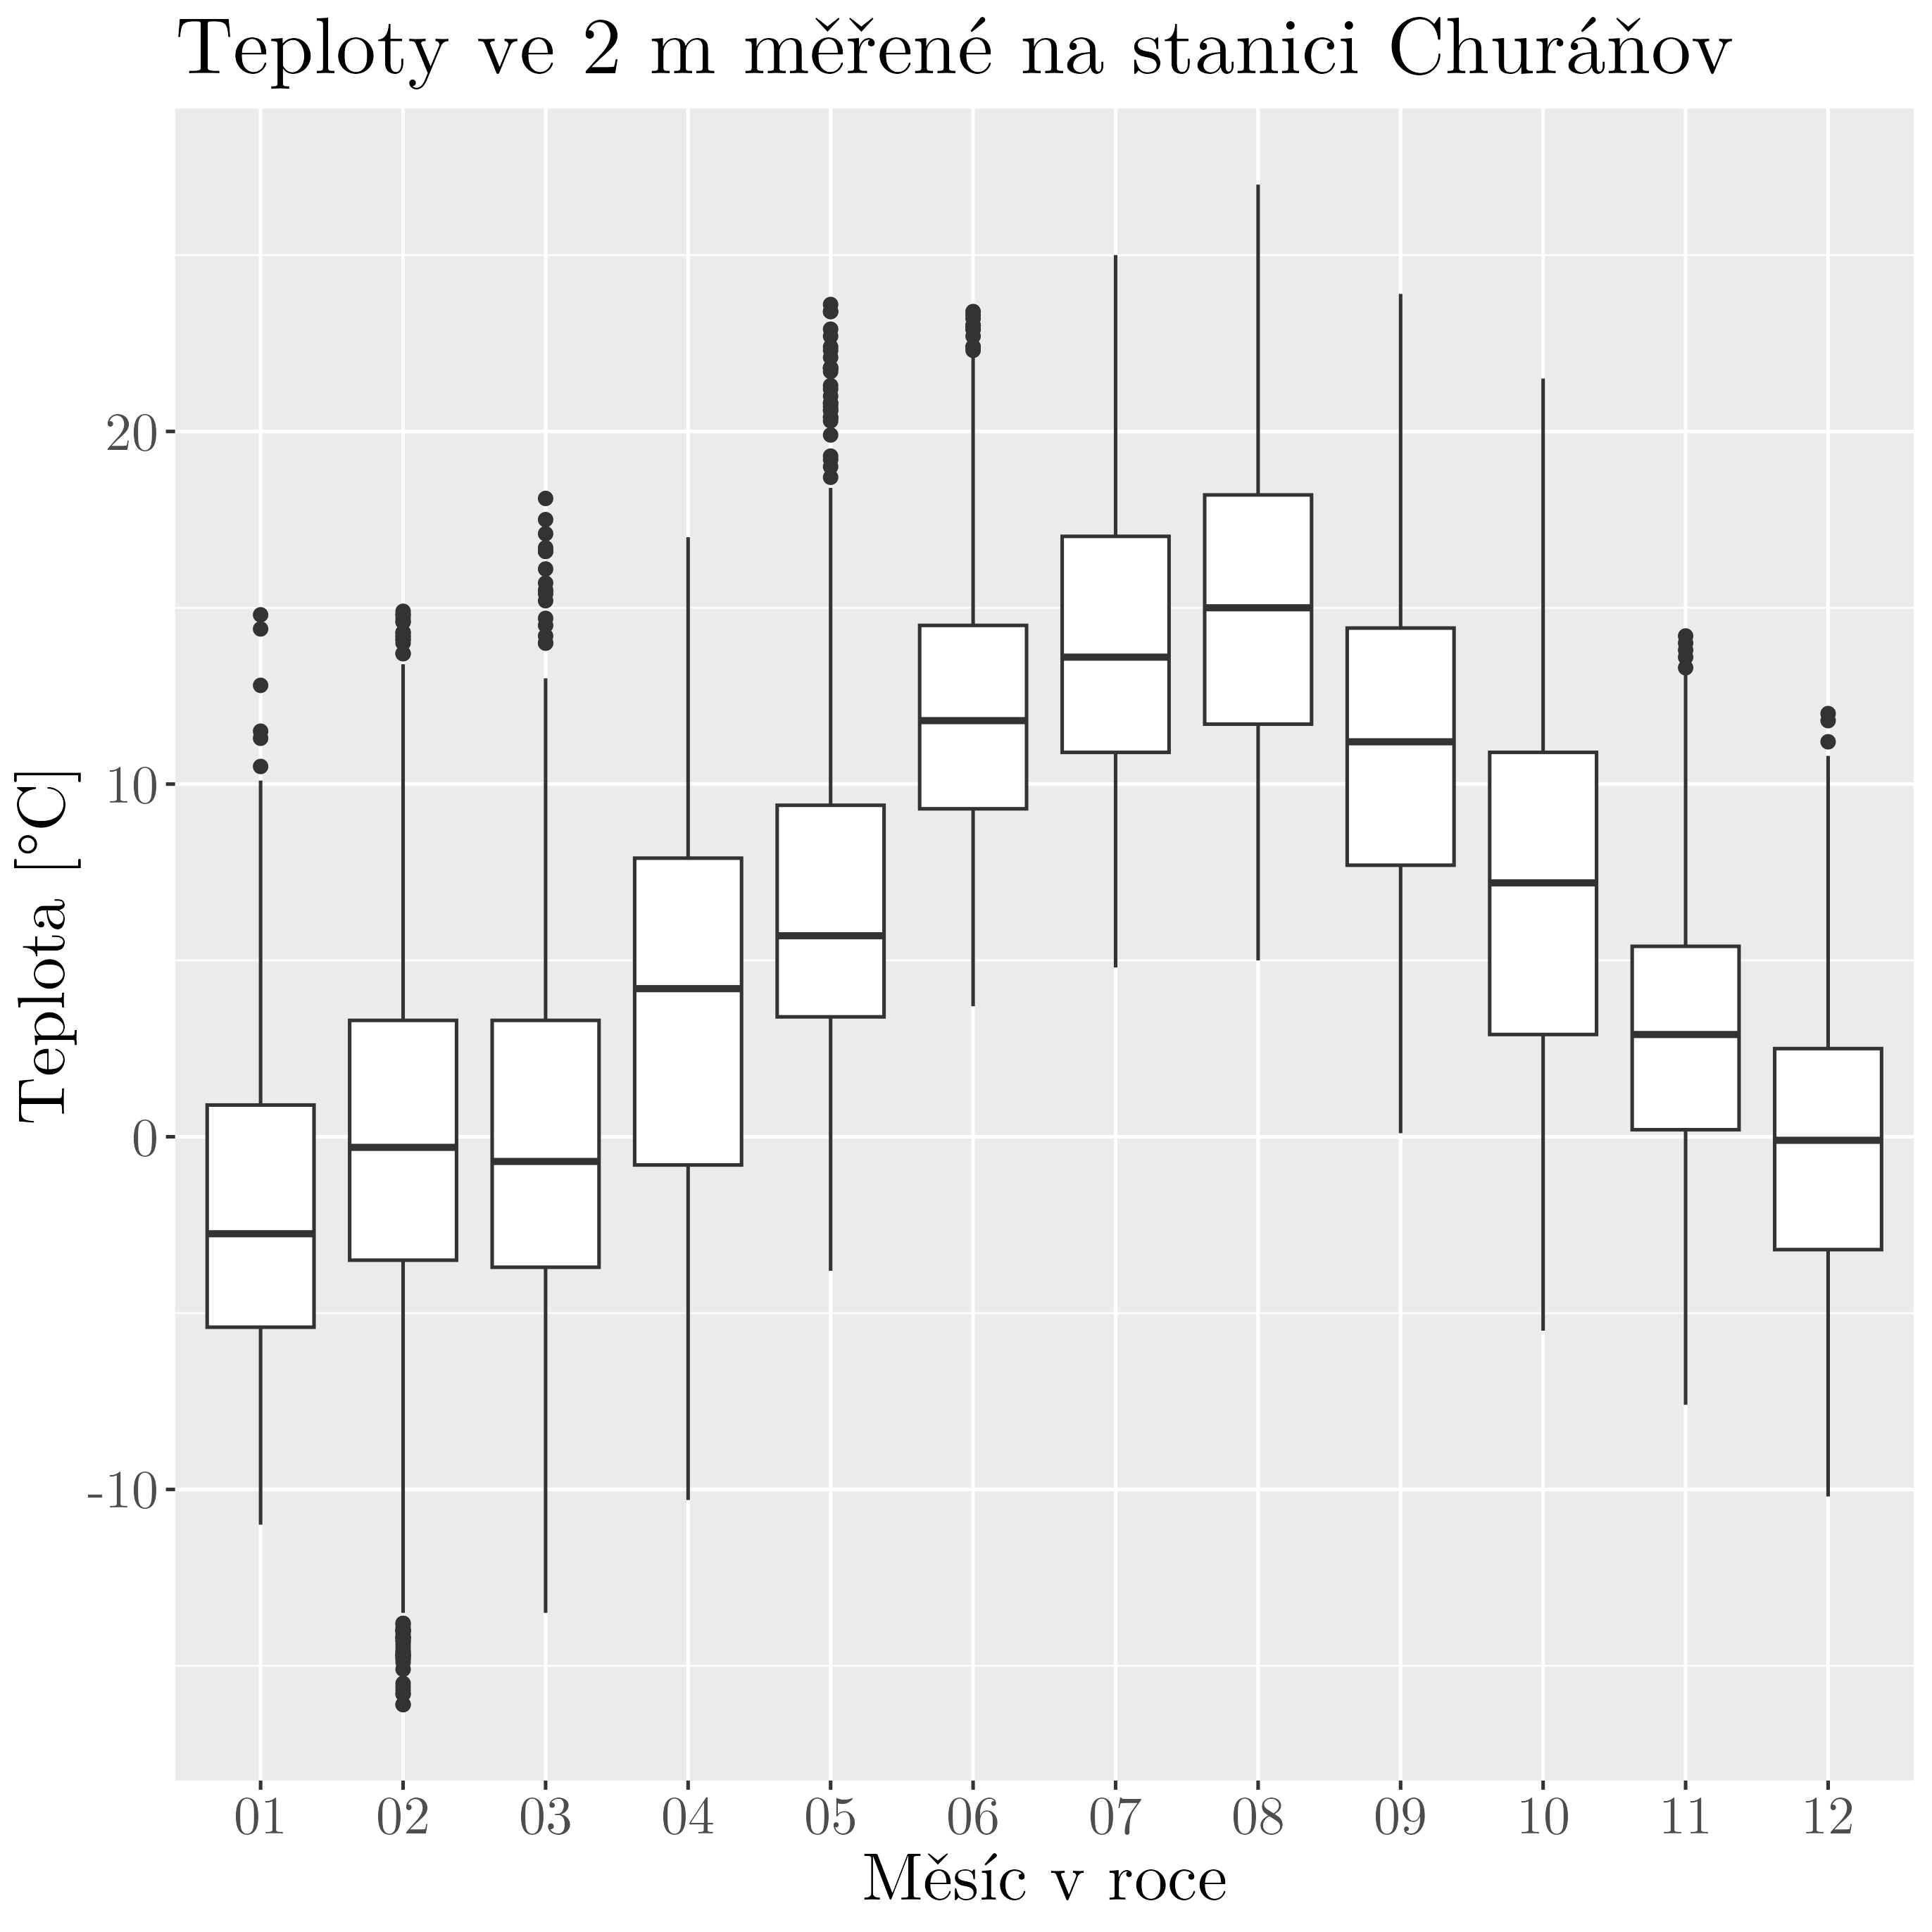
\includegraphics[width=\textwidth]{img/synop_temperature.png}
		\caption{}
		\label{fig:synop_temperature}
	\end{subfigure}
	\hfill
	\begin{subfigure}{0.45\textwidth}
  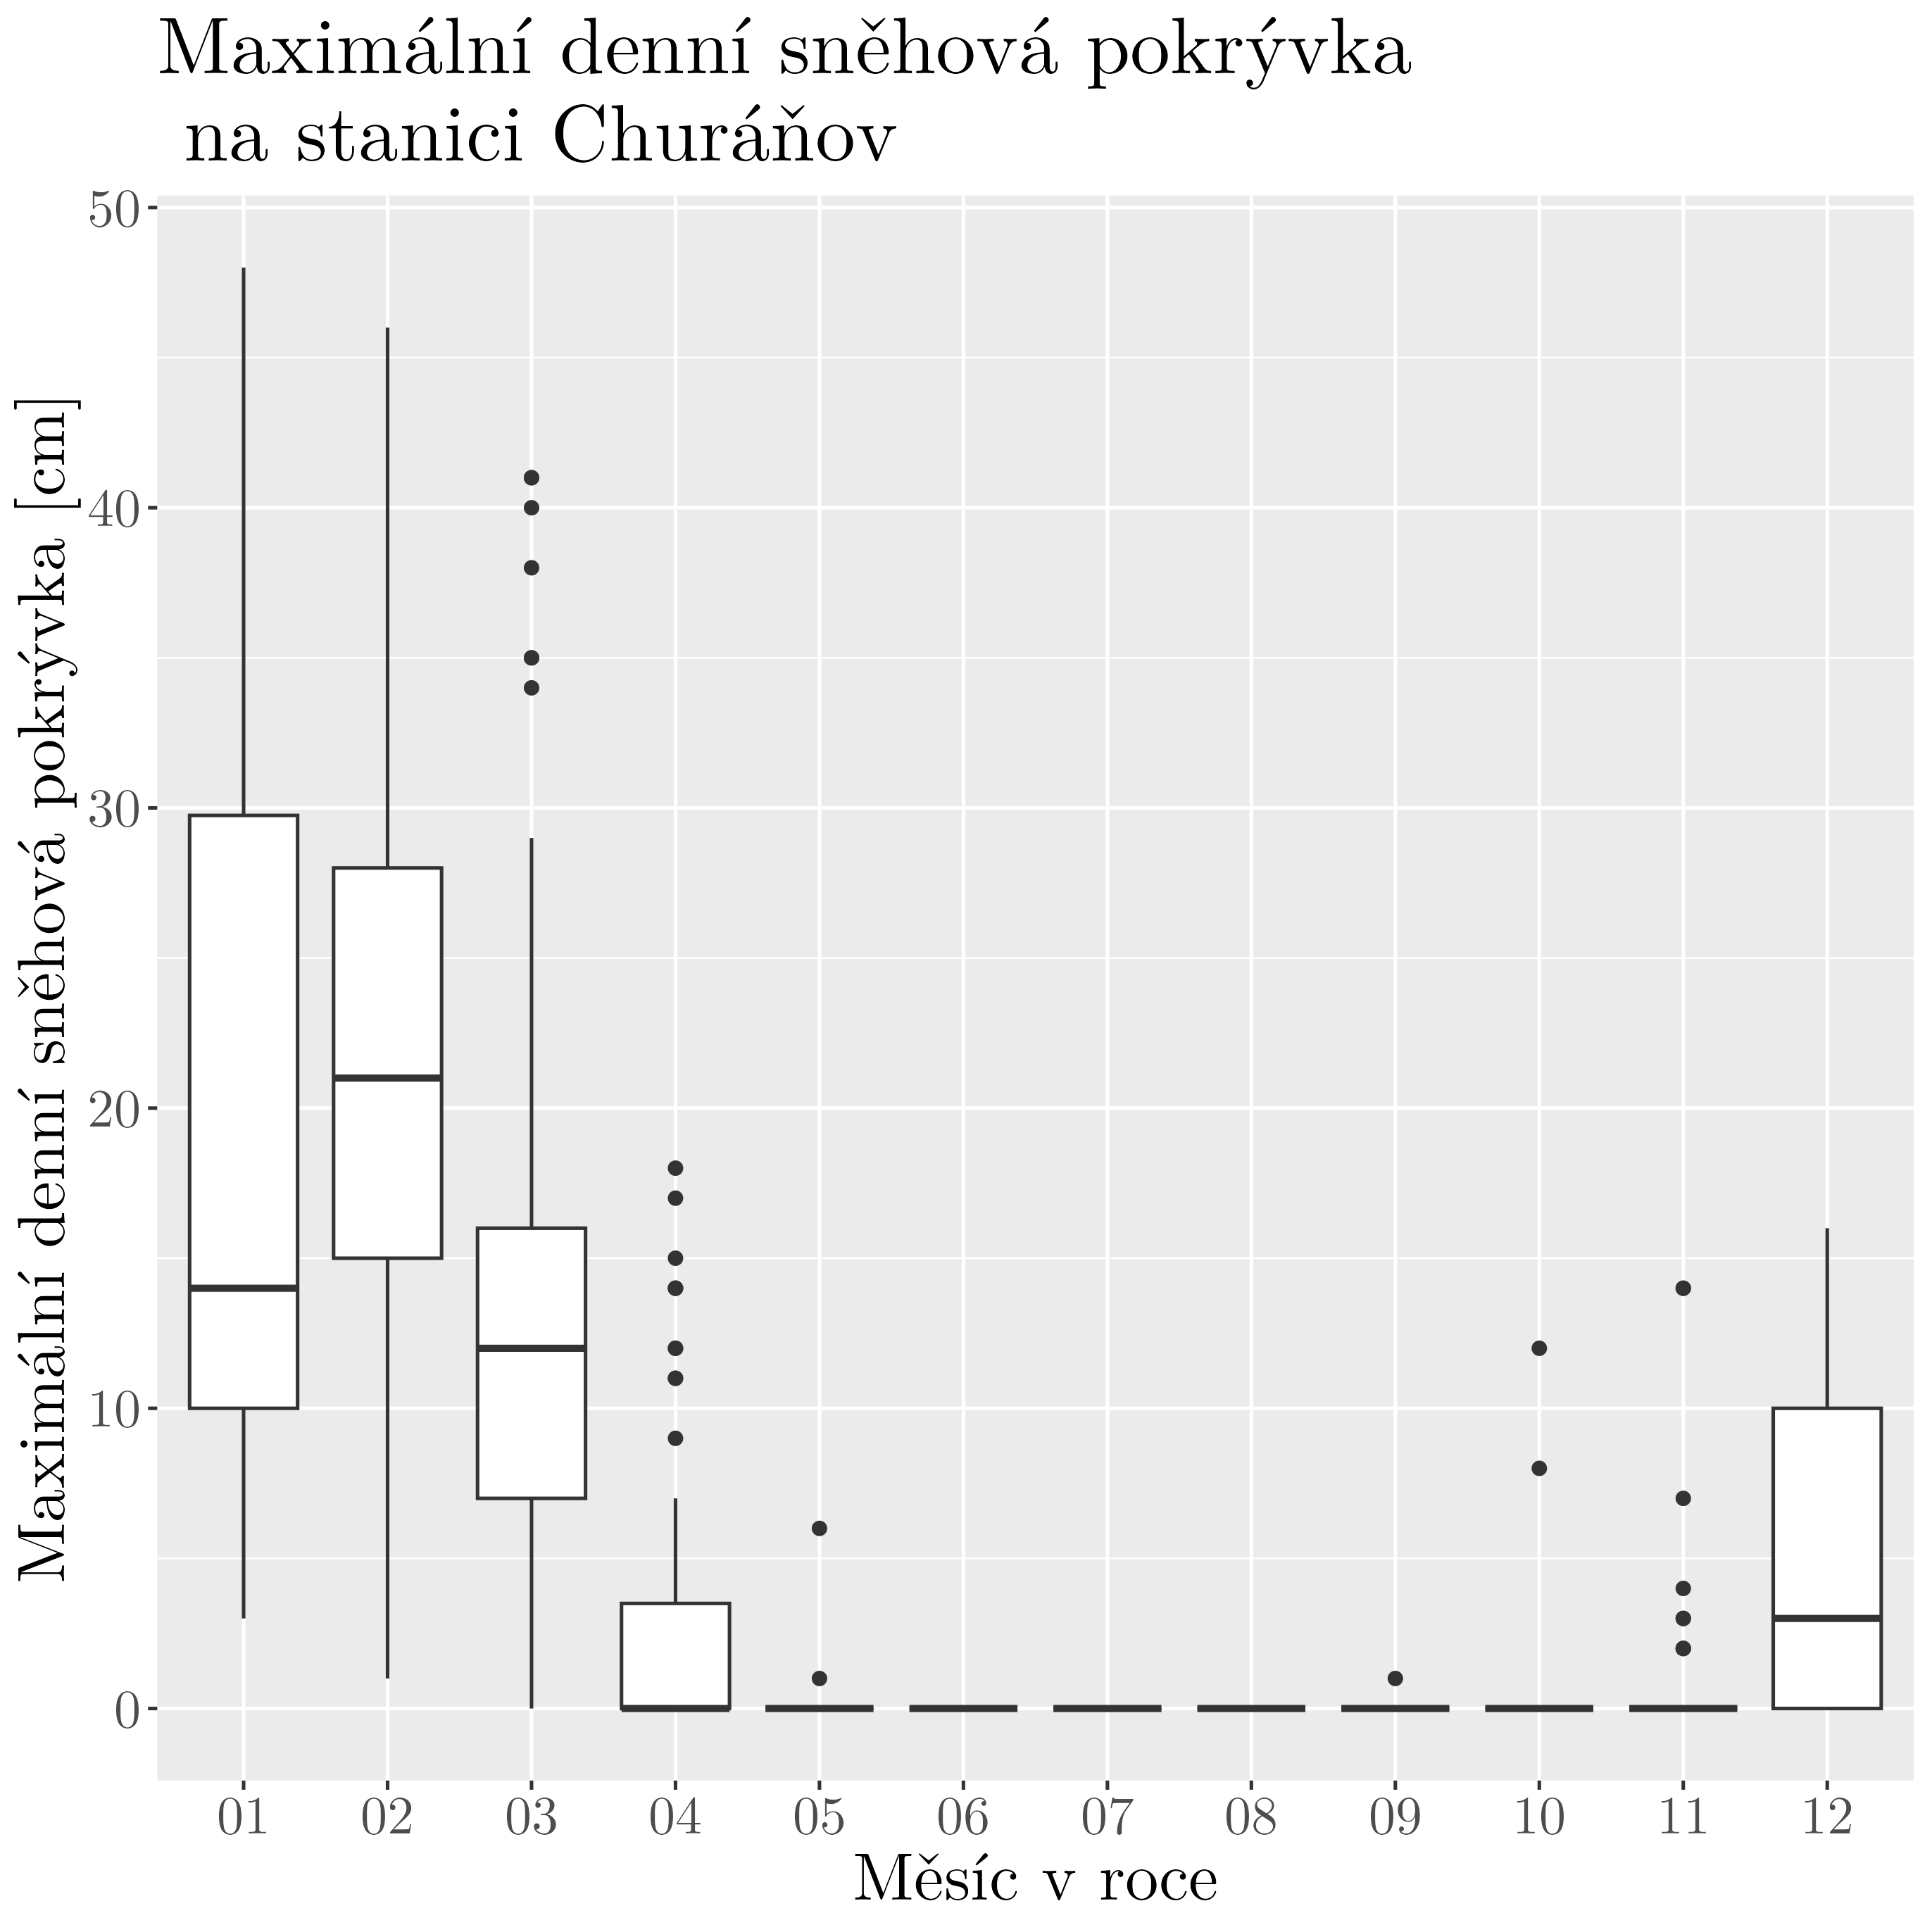
\includegraphics[width=\textwidth]{img/synop_snowcm.png}
		\caption{}
		\label{fig:synop_snowcm}
	\end{subfigure}
	\hfill
	\begin{subfigure}{0.45\textwidth}
  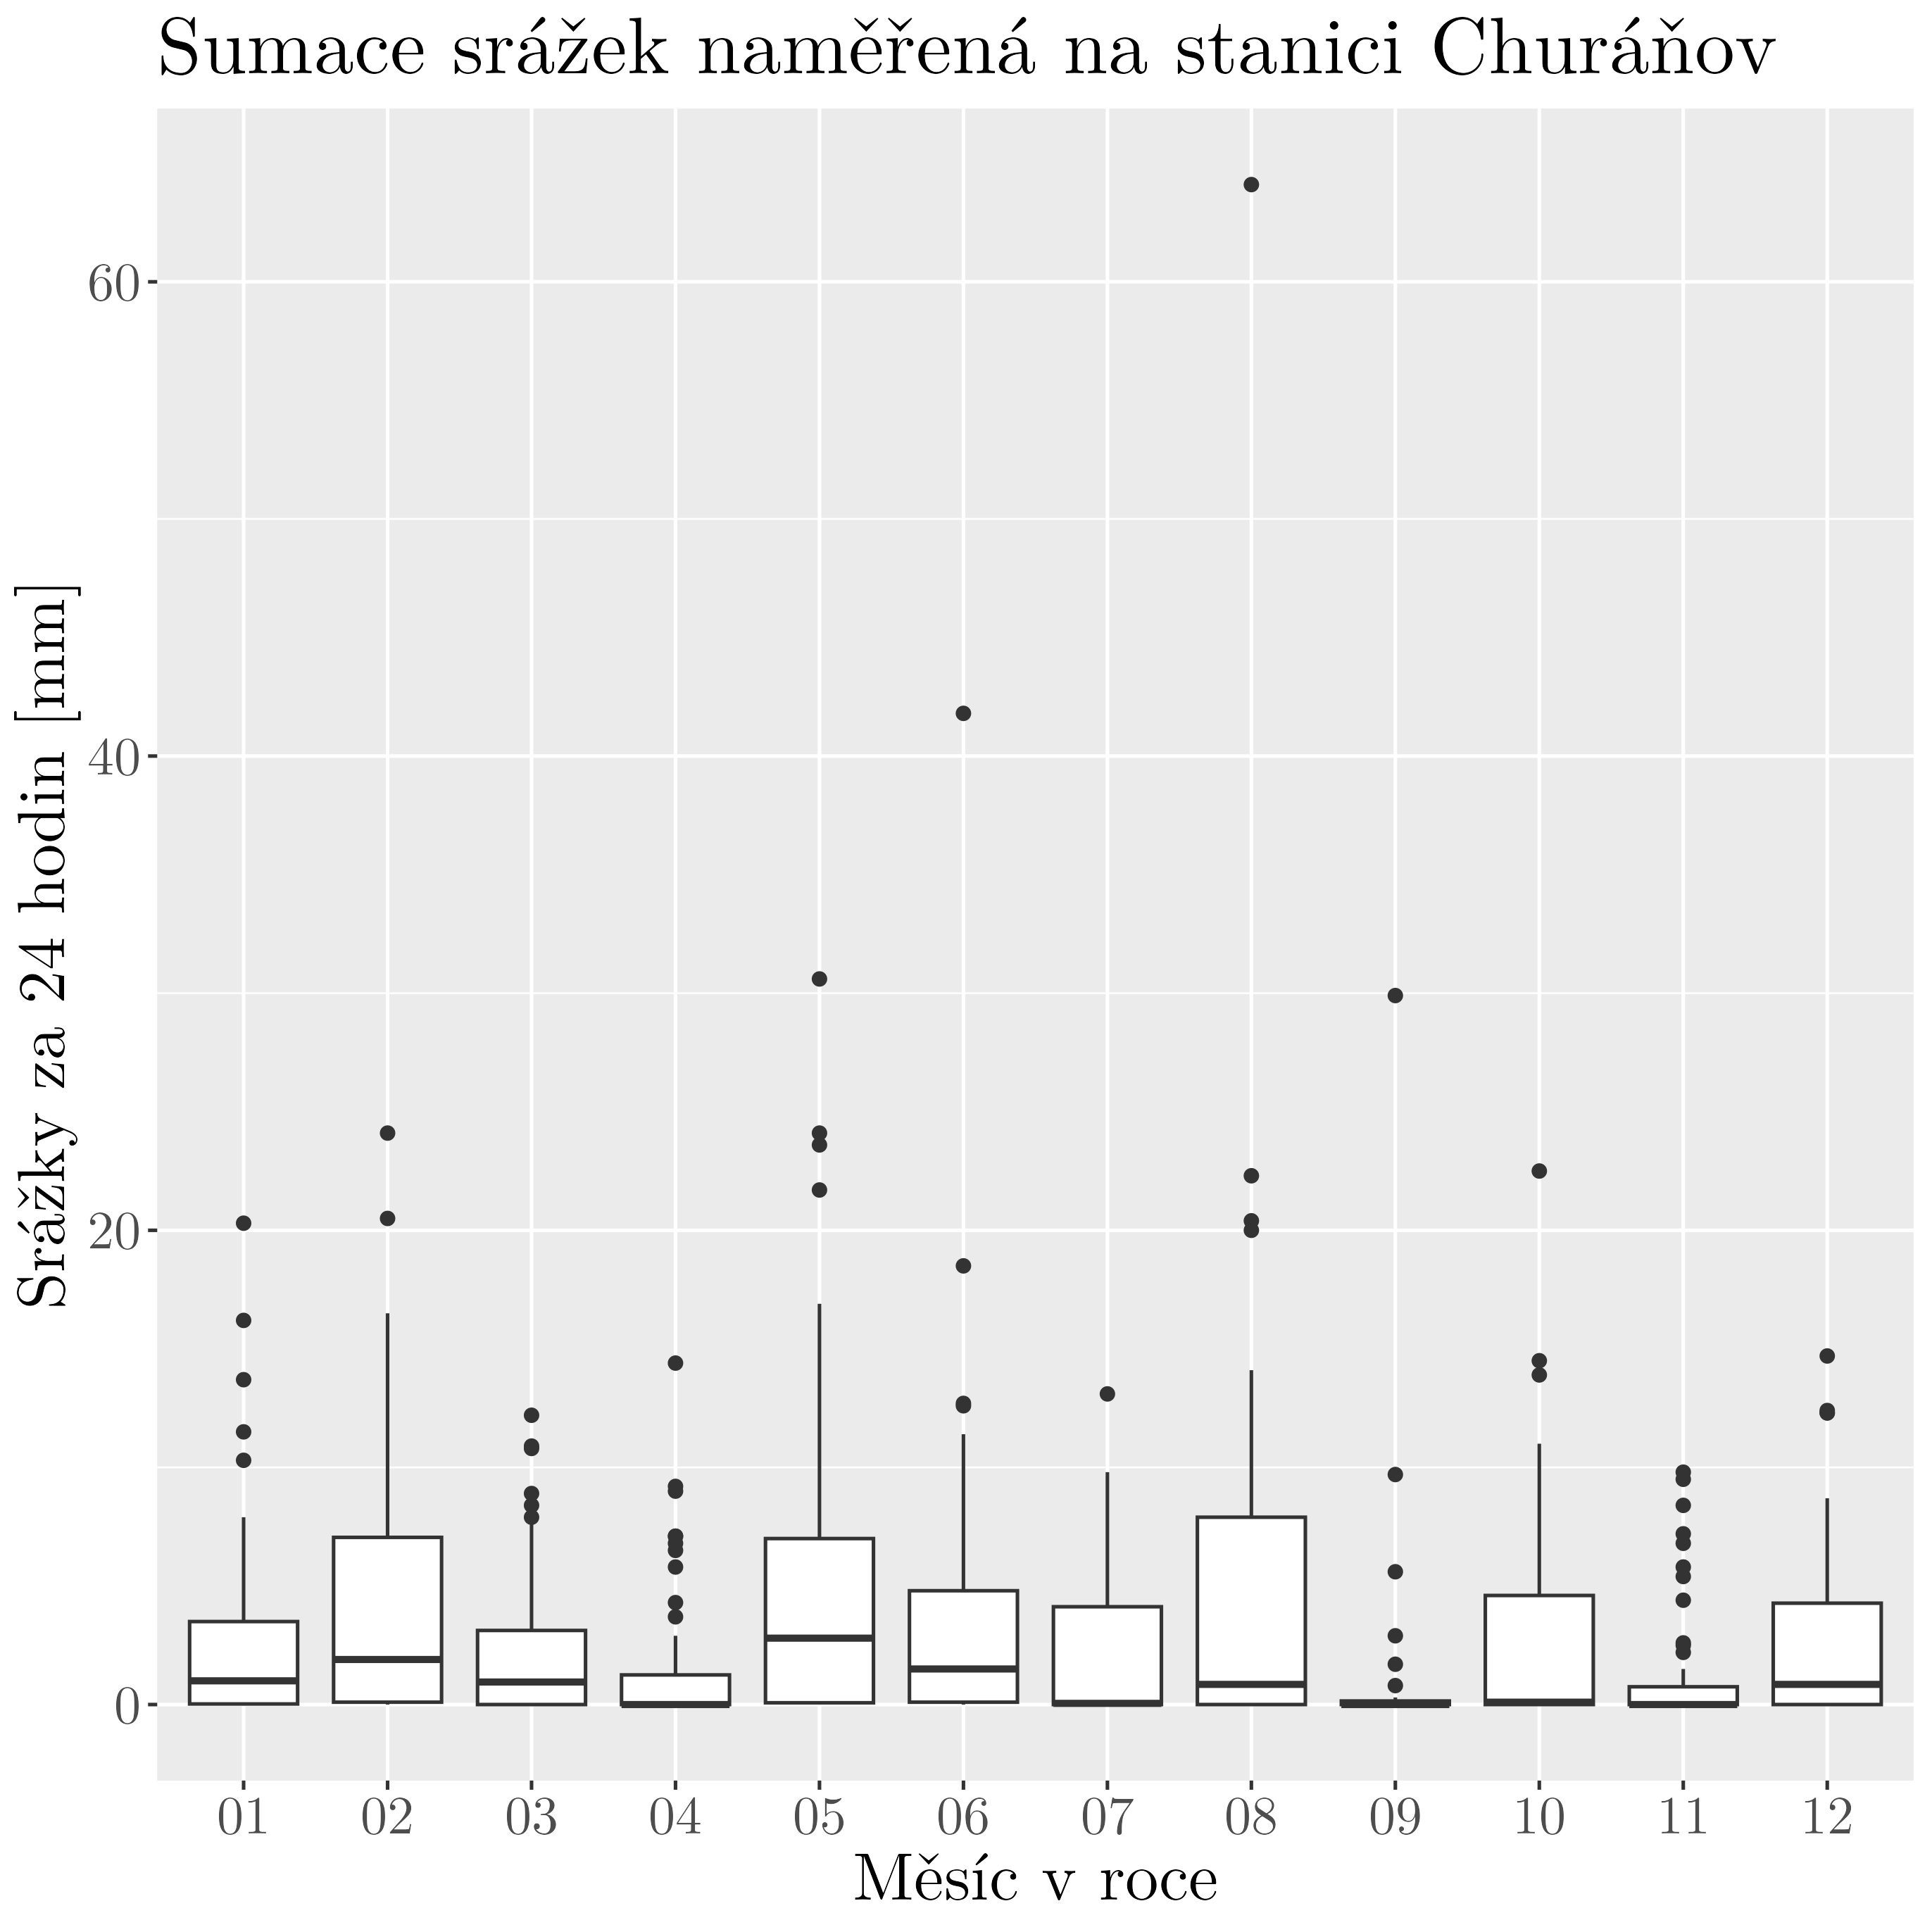
\includegraphics[width=\textwidth]{img/synop_prec.png}
		\caption{}
		\label{fig:synop_prec}
	\end{subfigure}
	\hfill
	\begin{subfigure}{0.45\textwidth}
  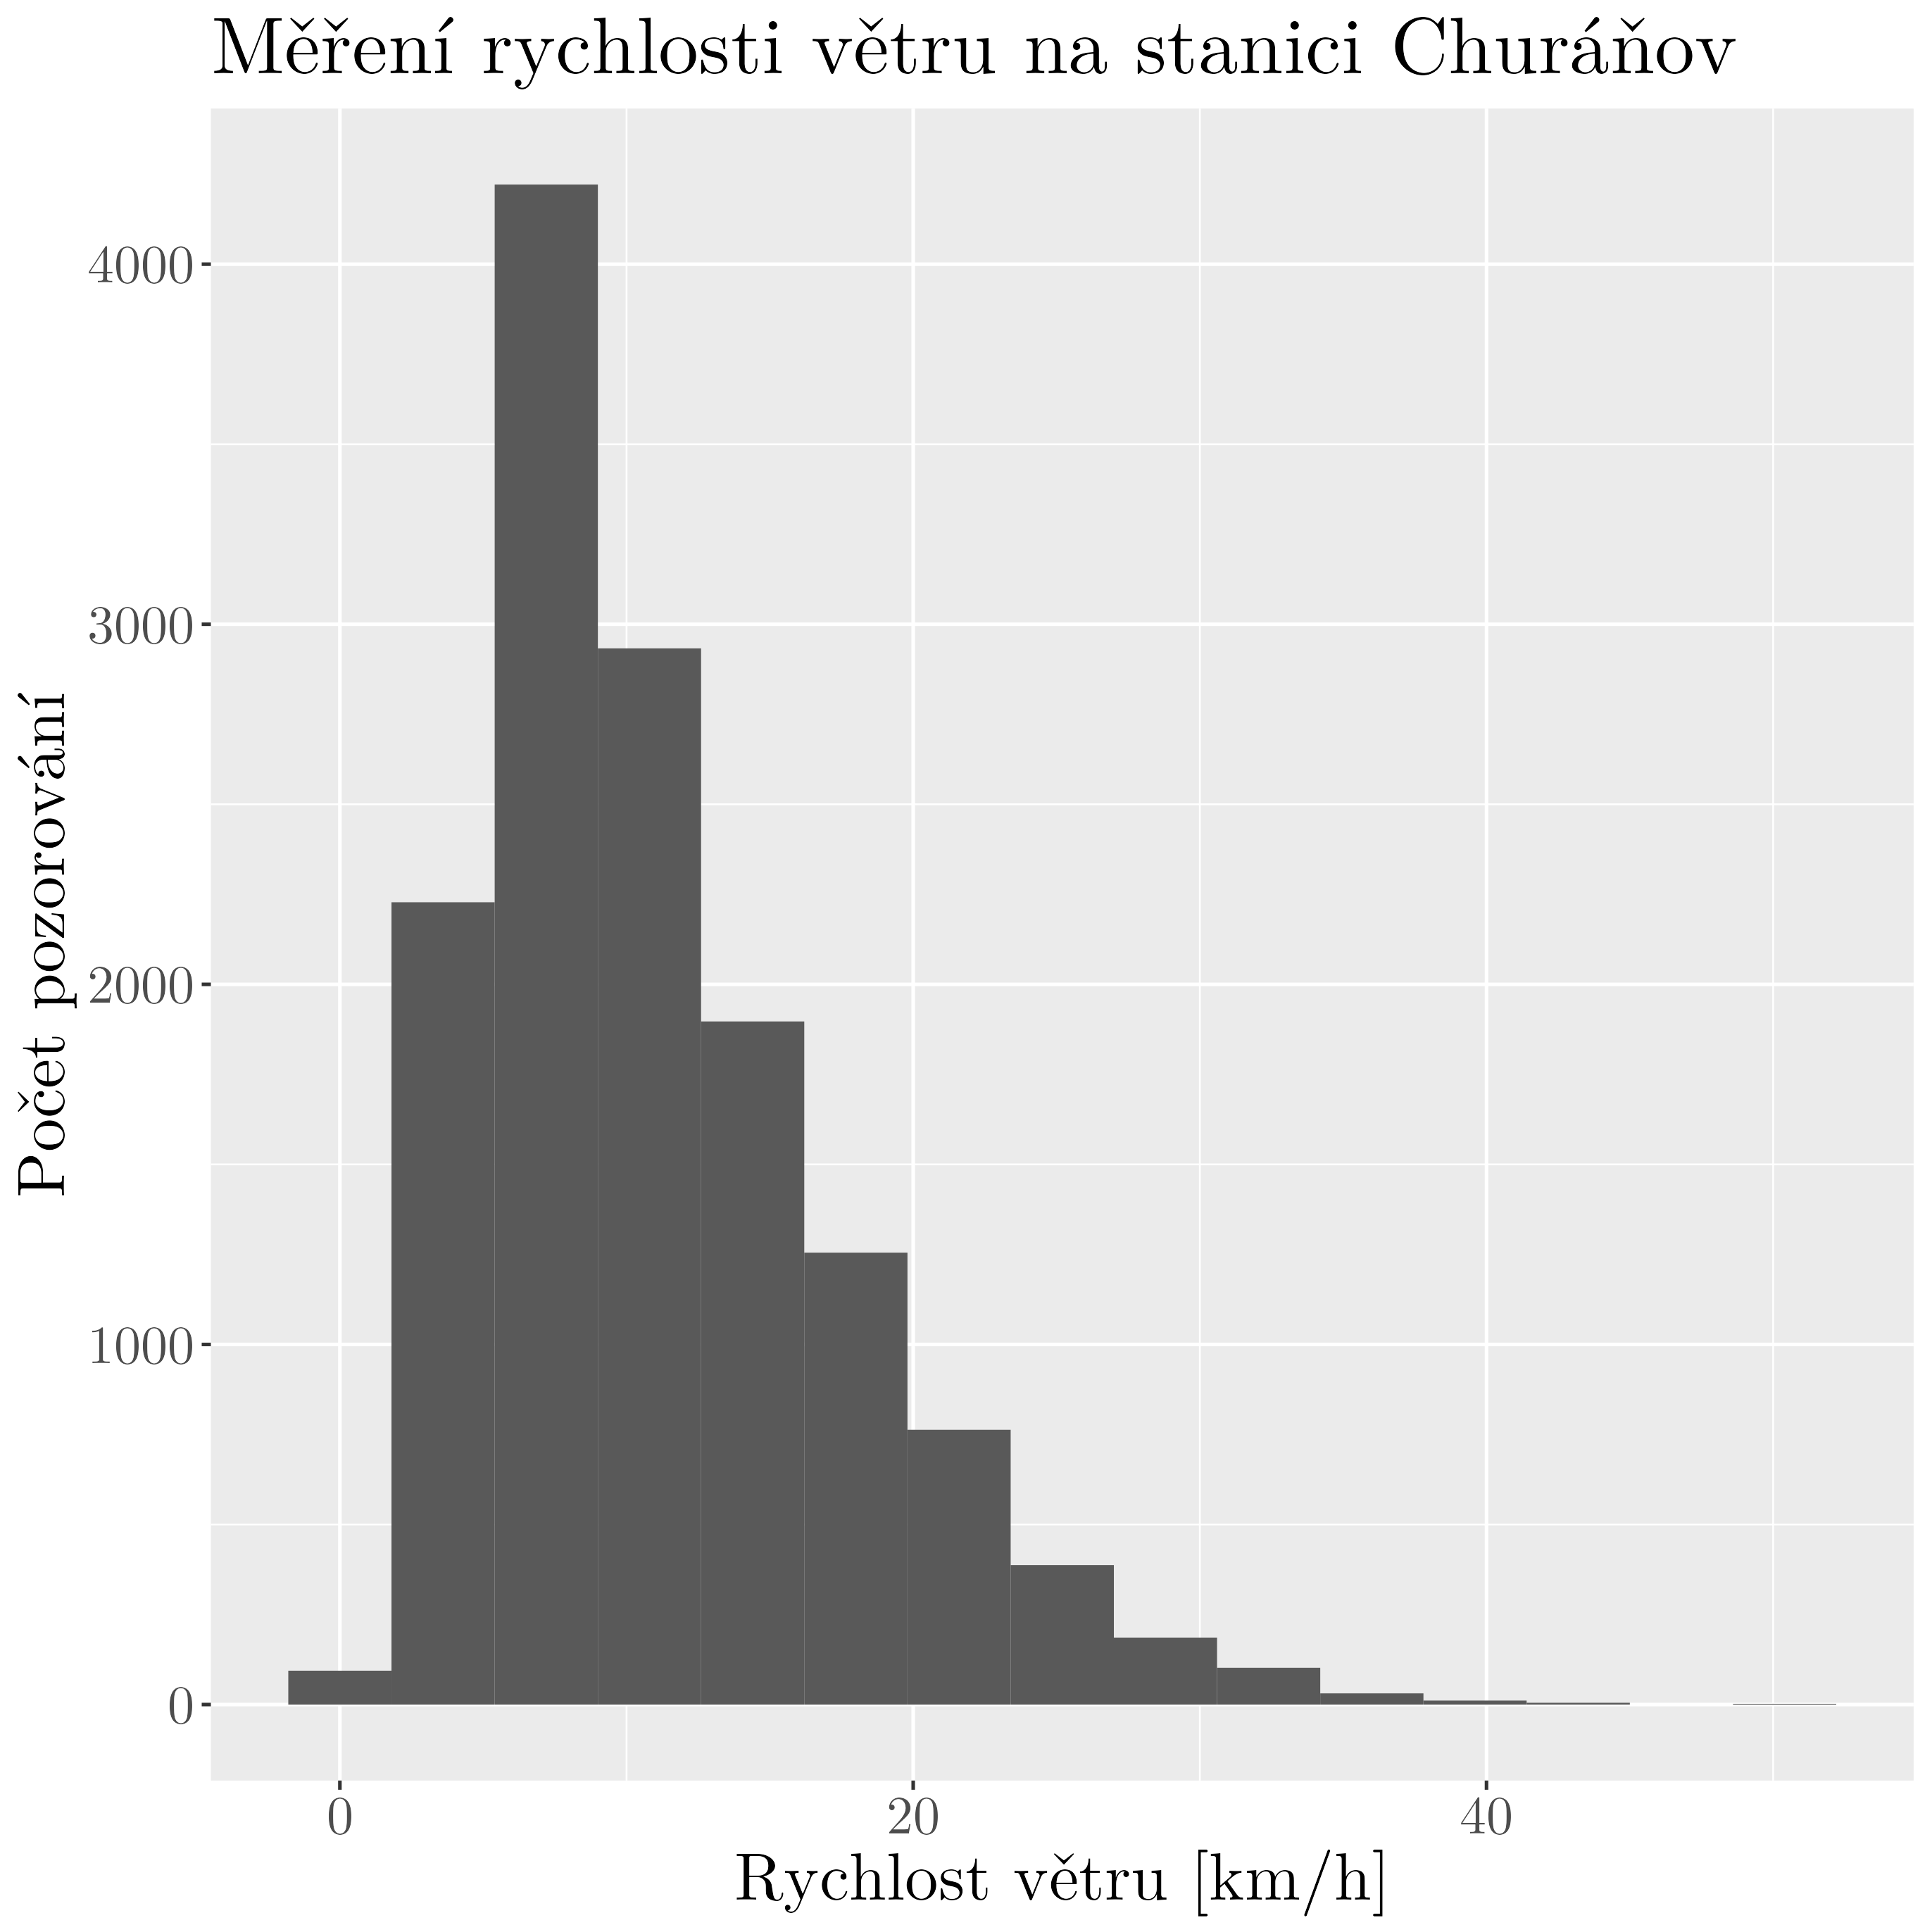
\includegraphics[width=\textwidth]{img/synop_ffkmh.png}
		\caption{}
		\label{fig:synop_ffkmh}
	\end{subfigure}
	\caption{Data ze synoptické stanice Churáňov za období 12.10.2019 až 20.5.2021} 
	\label{fig:chmuukazka}
\end{figure}

\section{Data z BÚ AV}
Data poskytnutá Botanickým ústavem Akademie věd České republiky byla naměřená dvěma typy čidel popisovanými v \ref{chap:loggers}. V části o zpracování dat se budeme zabývat pouze těmi plochami, které jsou opatřeny jak pozemními čidly, tak čidly ve standartní výšce $\SI{2}{m}$. Na obrázku \ref{fig:rozlozenicidel} můžeme vidět jejich prostorové rozložení, celkově jde o 157 čidel. 

Umístění čidel bylo vybíráno tak aby pokryly gradienty nadmořské výšky (5 tříd), potenciální solární radiace (3 třídy) a topografického vlhkostního indexu (3 třídy). Plochy byly dále doplněny tak, aby bylo rovnoměrně pokryto území národních parků a aby se nevyskytovaly poblíž turistických stezek.

\begin{figure}
	\centering
	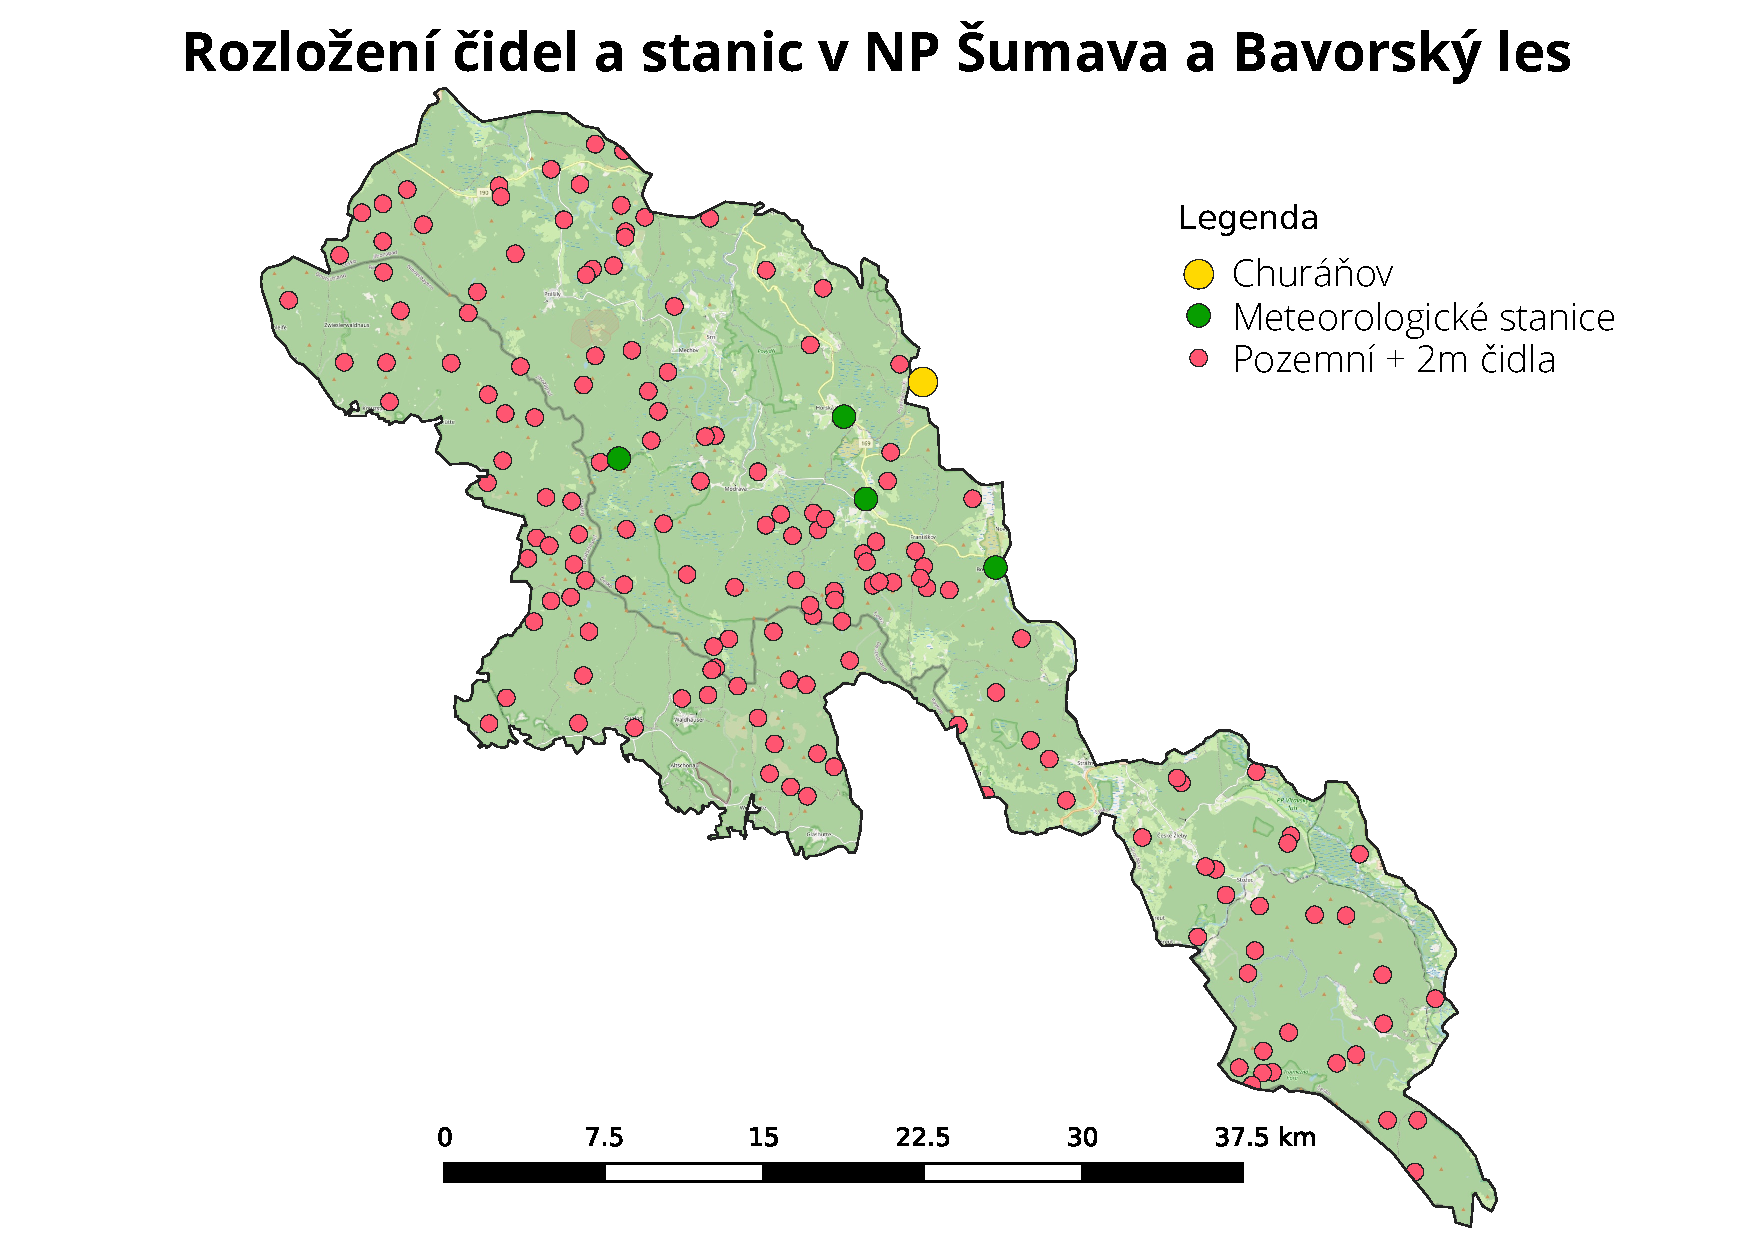
\includegraphics[width=0.95\textwidth]{img/rozlozenicidel.pdf}
	\caption{Rozložení čidel a meteorologický stanic napříč Národním parkem Šumava ($N=112$) a Národním parkem Bavorský les ($N=45$)}
	\label{fig:rozlozenicidel}
\end{figure}

Data vykazují malou chybovost, duplicitní a chybějící záznamy byly vyřazeny. Dále byla data vizuálně překontrolována a části, kdy byla čidla např. povytažená ze země (pozná se podle hodnot půdní vlhkosti), byly nahrazeny hodnotami NA. Podobně pokud čidlo T1 spadlo ze stromu tak jsou hodnoty nahrazeny NA. Toto čištění dat provedli RNDr. Josef Brůna, Ph.D., doc. Ing. Jan Wild, Ph.D. a další s jejichž svolením jsou data využitá v této práci.

Dostupnost dat z čidel je vidět na obrázku \ref{fig:dostupnostdat}, vidíme zde dvě skupiny čidel, jedny, nacházející se v Národním parku Bavorský les mají dostupná data pro cca 400 dnů, zatímco čidla z Národního parku Šumava mají dostupná data pro téměř 600 dnů. Na obrázku \ref{fig:dostupnostdnu} vidíme pak na kolika čidlech jsou zastoupeny jednotlivé dny.

\begin{figure}
	\centering
	\begin{subfigure}{0.45\textwidth}
  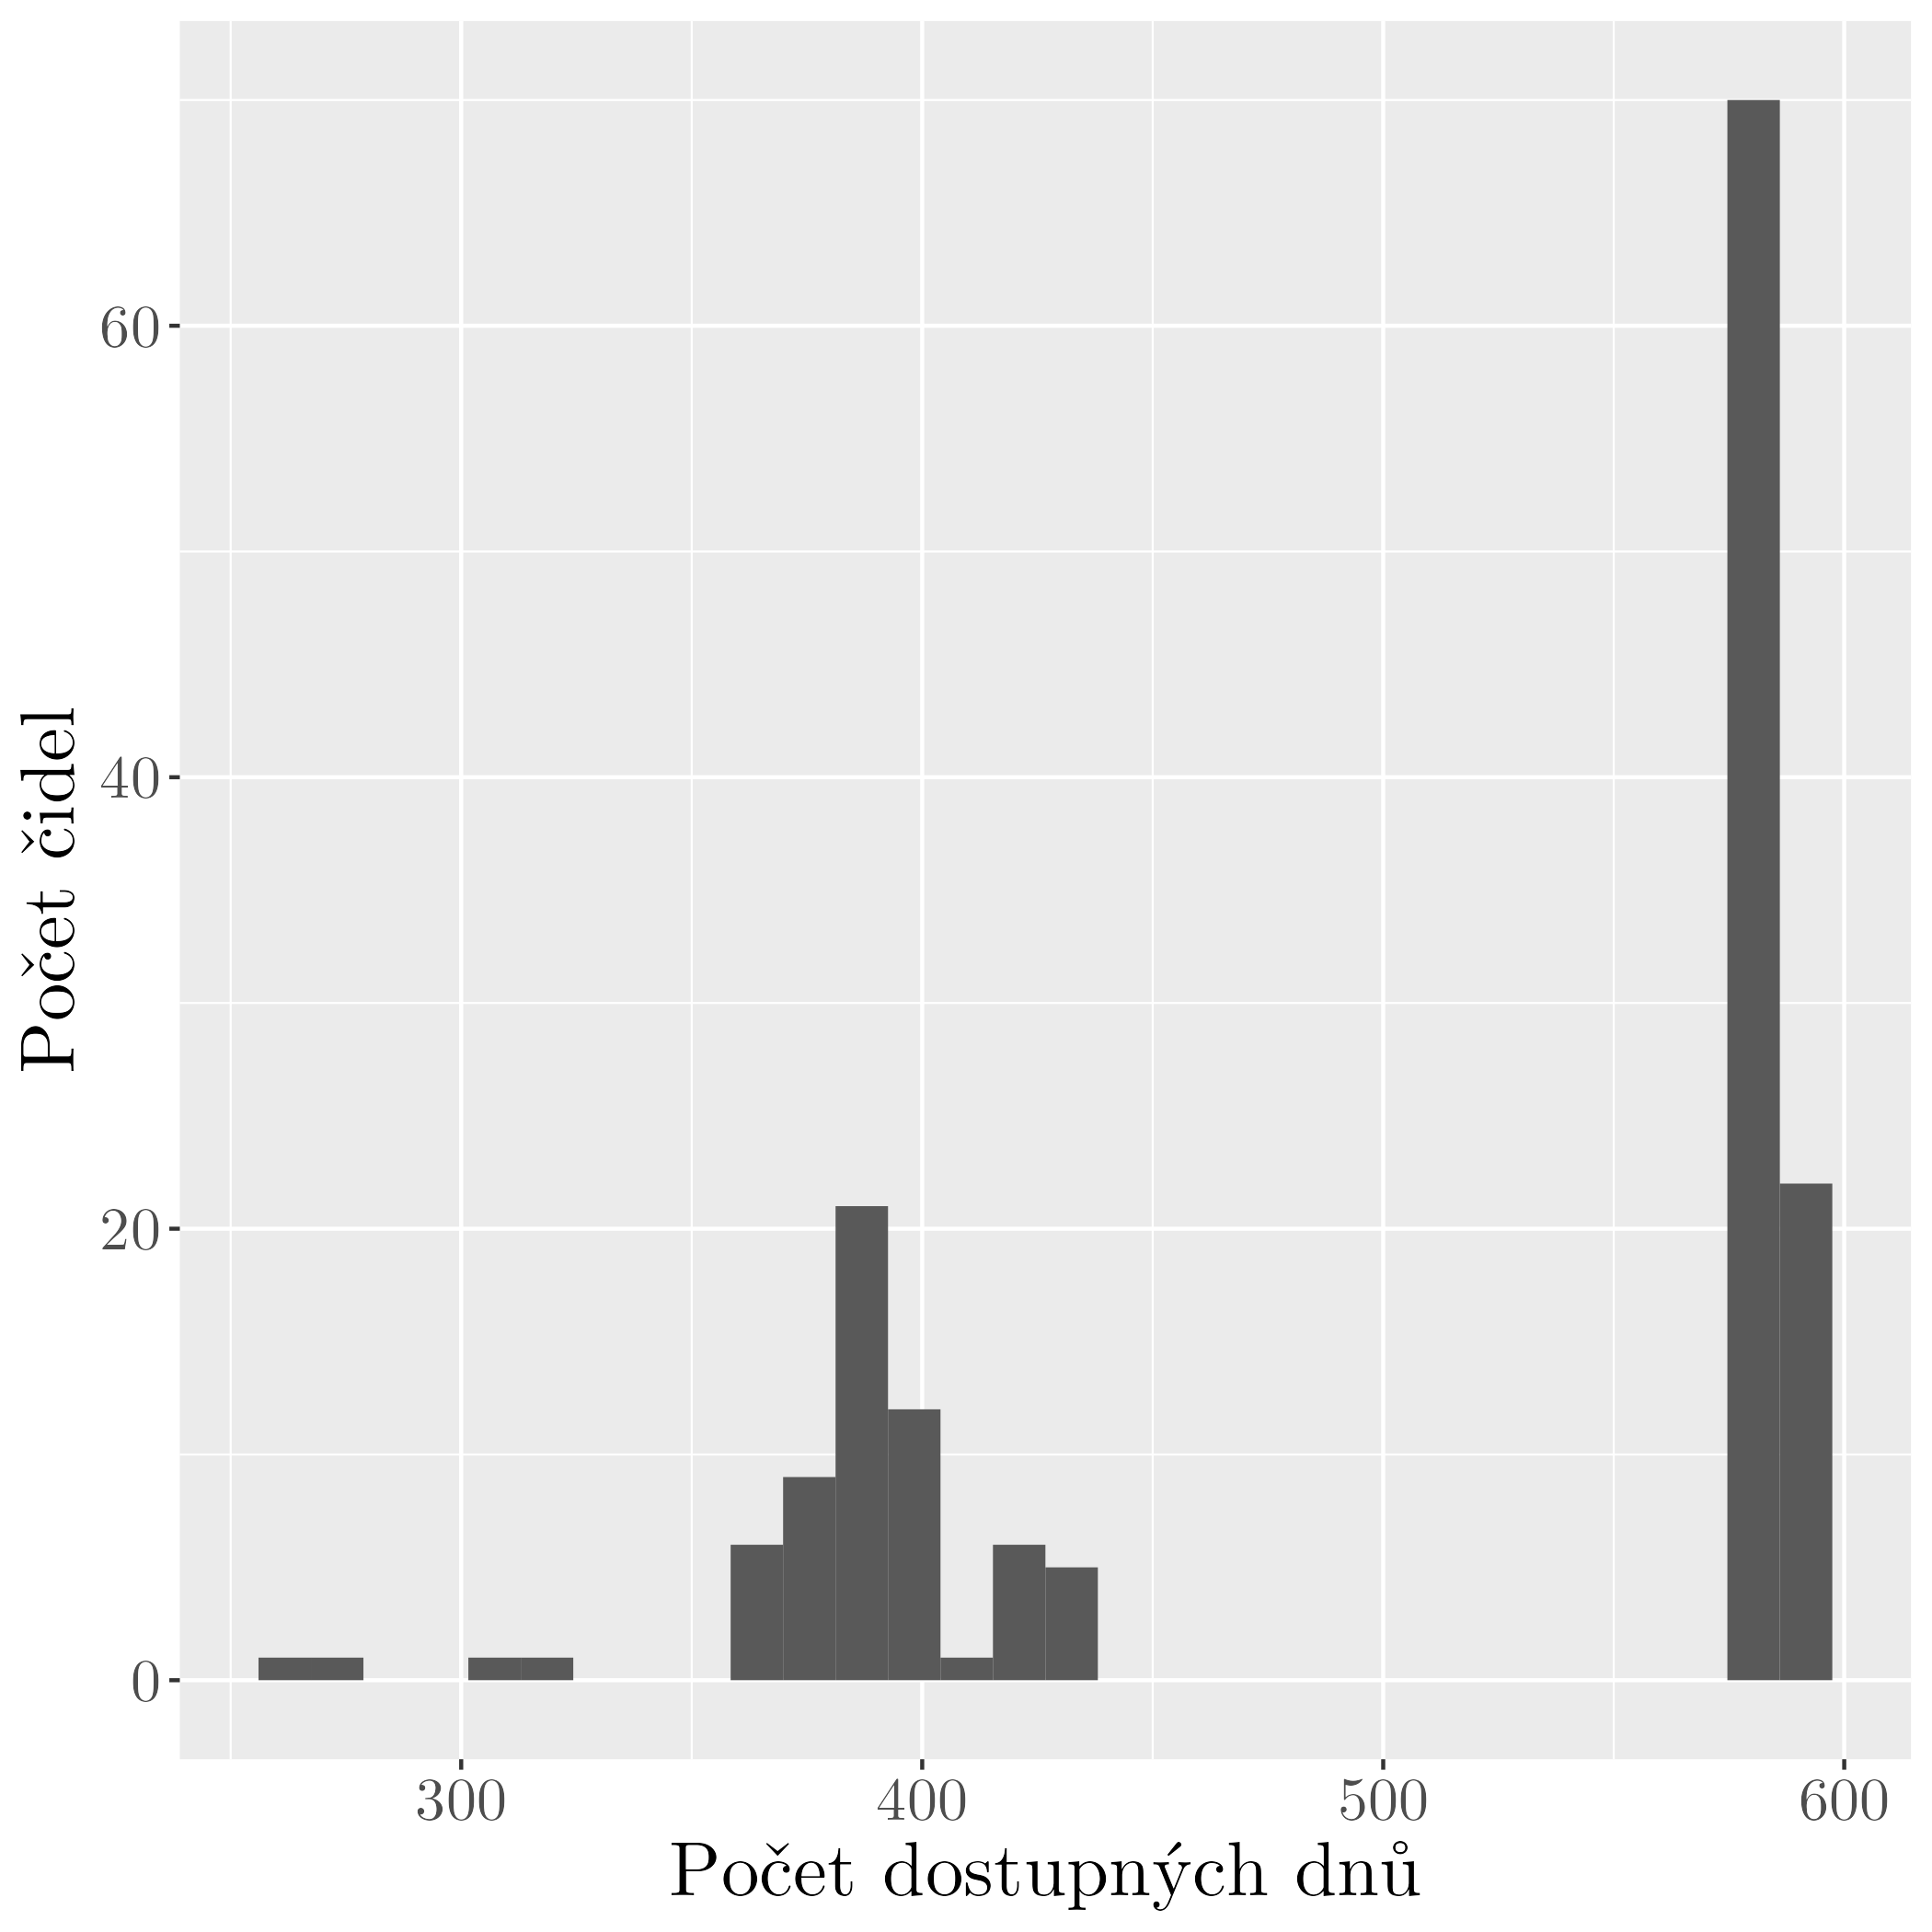
\includegraphics[width=\textwidth]{img/hist_numofdayavailability.png}
	\caption{Histogram ukazující množství dostupných dnů pro jednotlivá čidla}
	\label{fig:dostupnostdat}
	\end{subfigure}
	\hfill
	\begin{subfigure}{0.45\textwidth}
  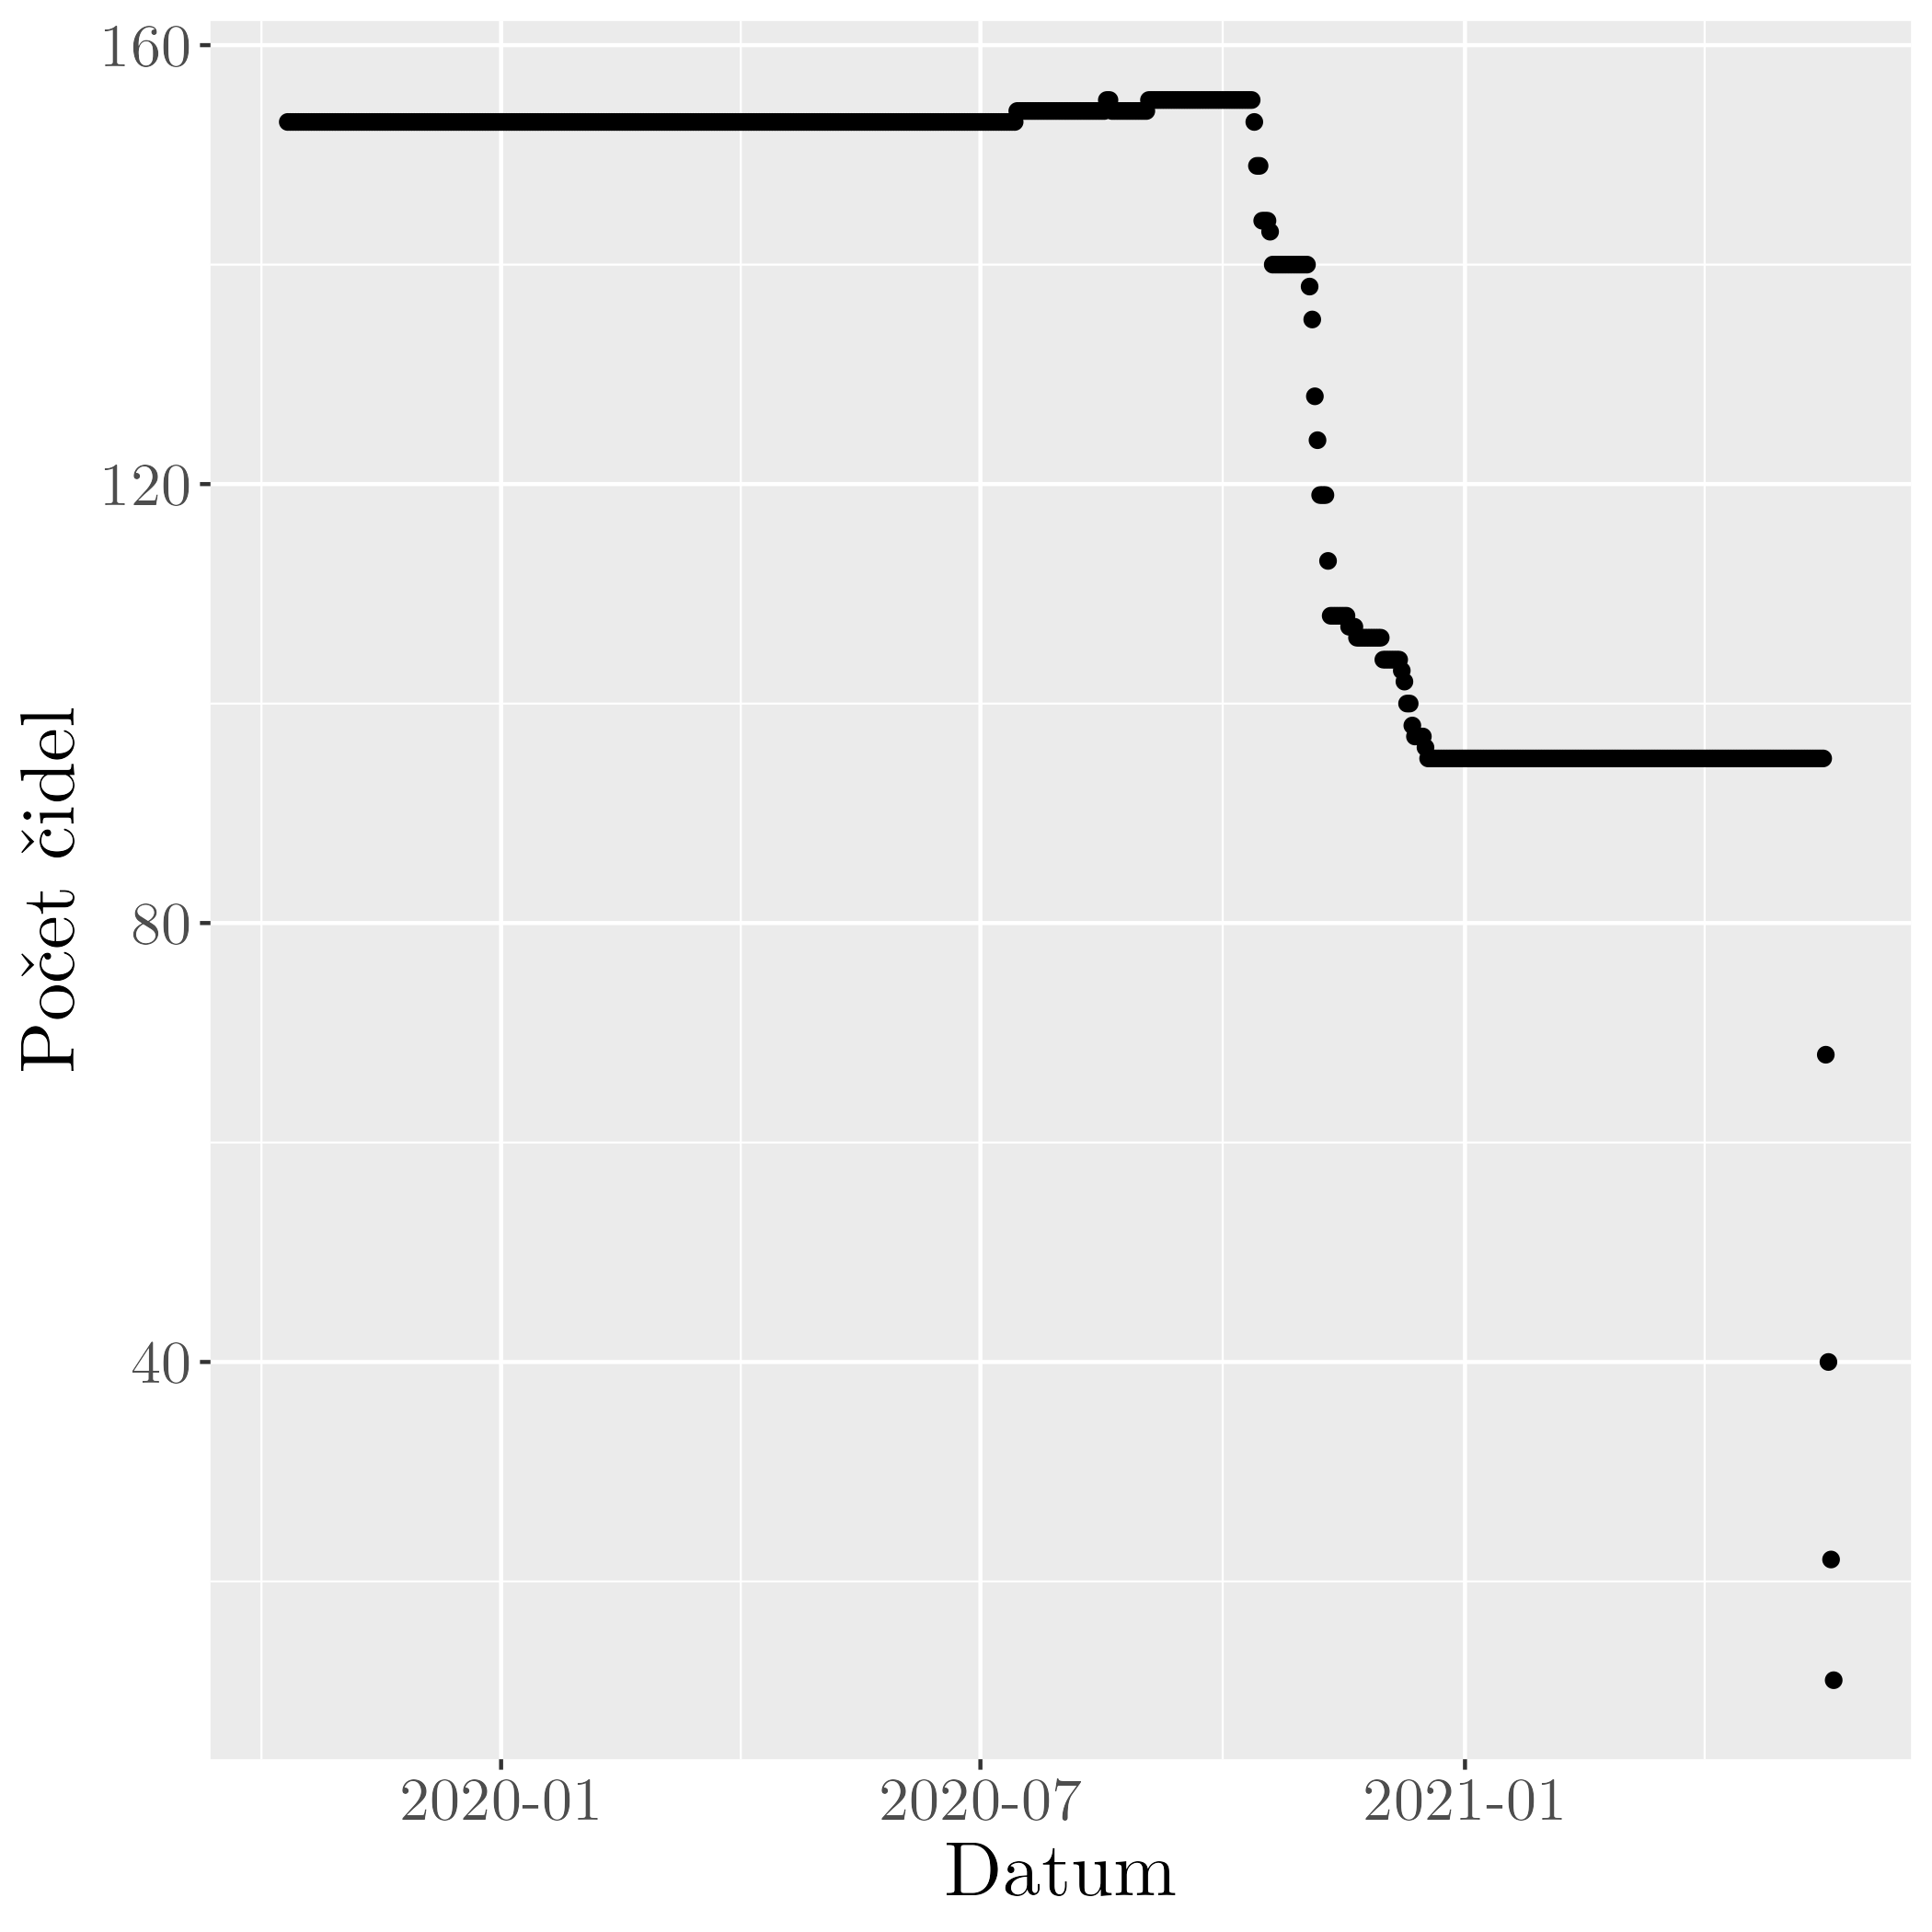
\includegraphics[width=\textwidth]{img/date_availability.png}
	\caption{Graf zastoupení čidel pro jednotlivé dny}
	\label{fig:dostupnostdnu}
	\end{subfigure}
	\caption{Dostupnost dat z čidel}
\end{figure}

\section{Ukázky použitých dat}
Dále se podívejme na ukázku dat naměřených na čidlech. Na obrázcích \ref{fig:hours} můžeme vidět kdy nastávaly maximální a minimální teploty ve výškách $\SI{0}{cm}$ a $\SI{15}{cm}$ nad zemí, denní hodina je uvedená v UTC, nikoliv SEČ nebo SELČ. U maximálních teplot si můžeme všimnout kromě maxima v okolí 10 UTC také menšího maxima a odlehlých hodnot způsobených přítomností sněhu v zimě. Podobně měl sníh vliv i na dobu minimálních teplot v zimě.

\begin{figure}
	\centering
	\begin{subfigure}{0.45\textwidth}
  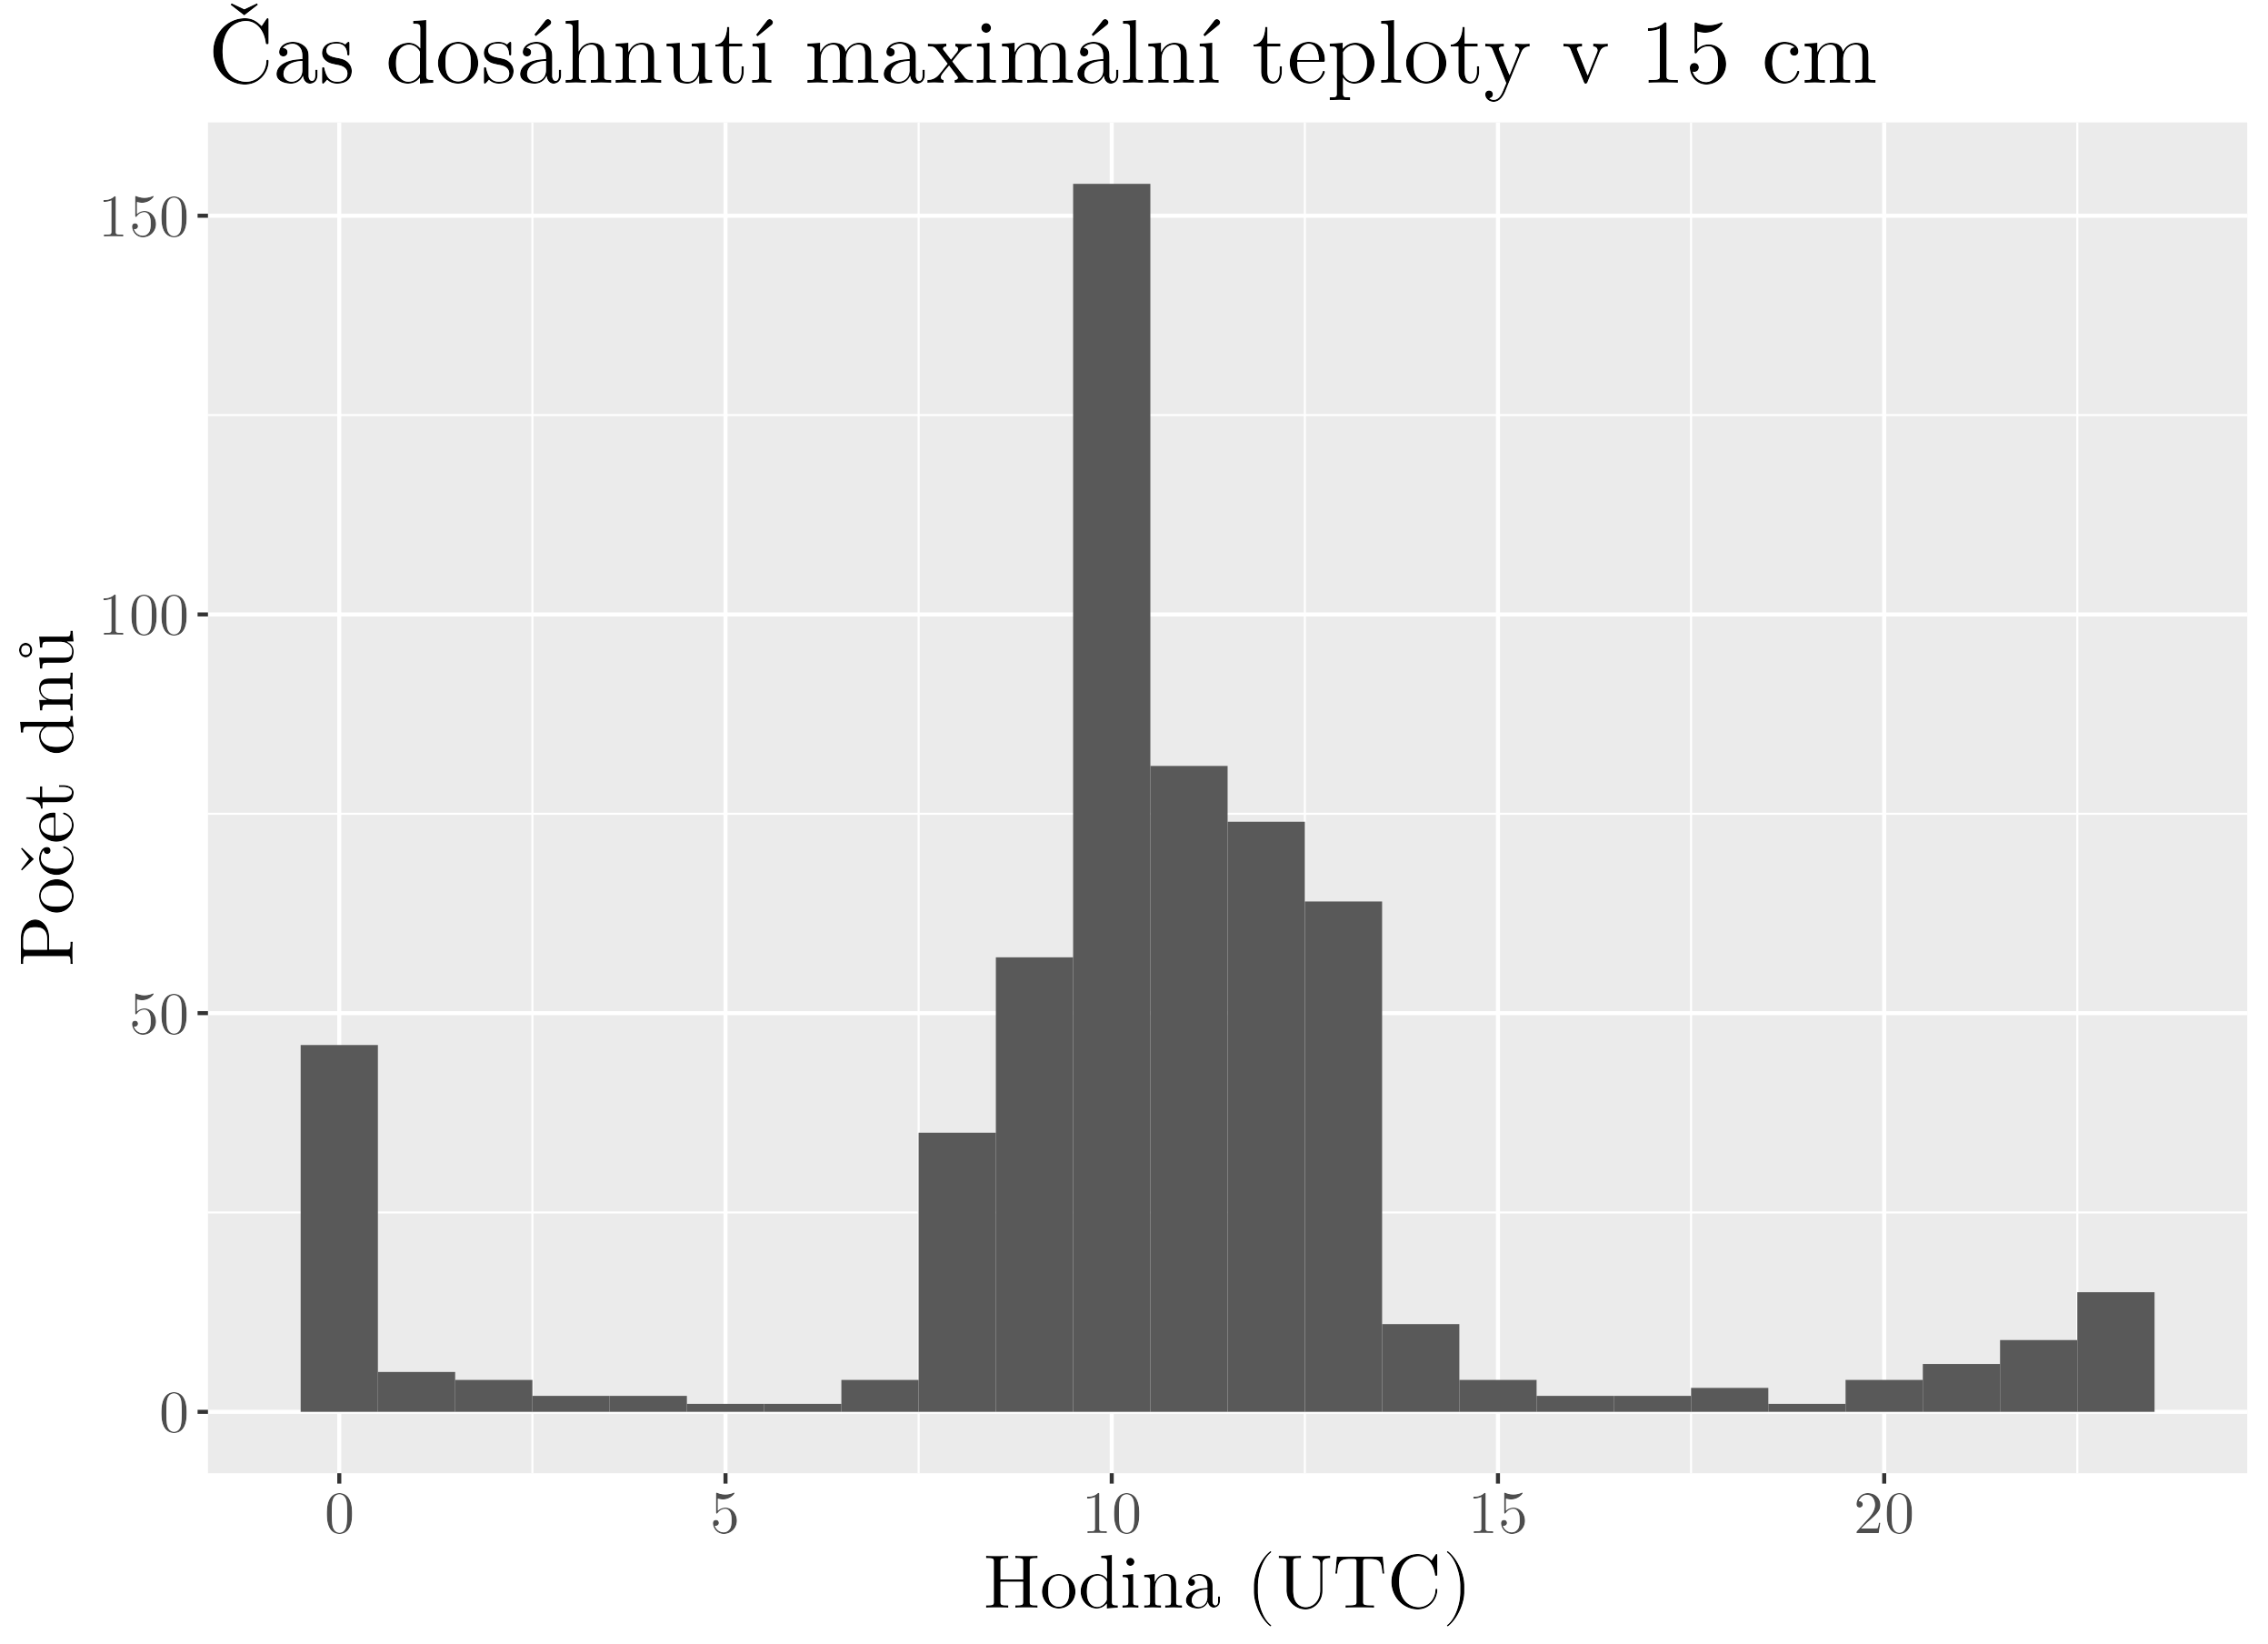
\includegraphics[width=\textwidth]{img/hist_hourmax15cm.png}
		\caption{}
		\label{fig:hourmax15cm}
	\end{subfigure}
	\hfill
	\begin{subfigure}{0.45\textwidth}
  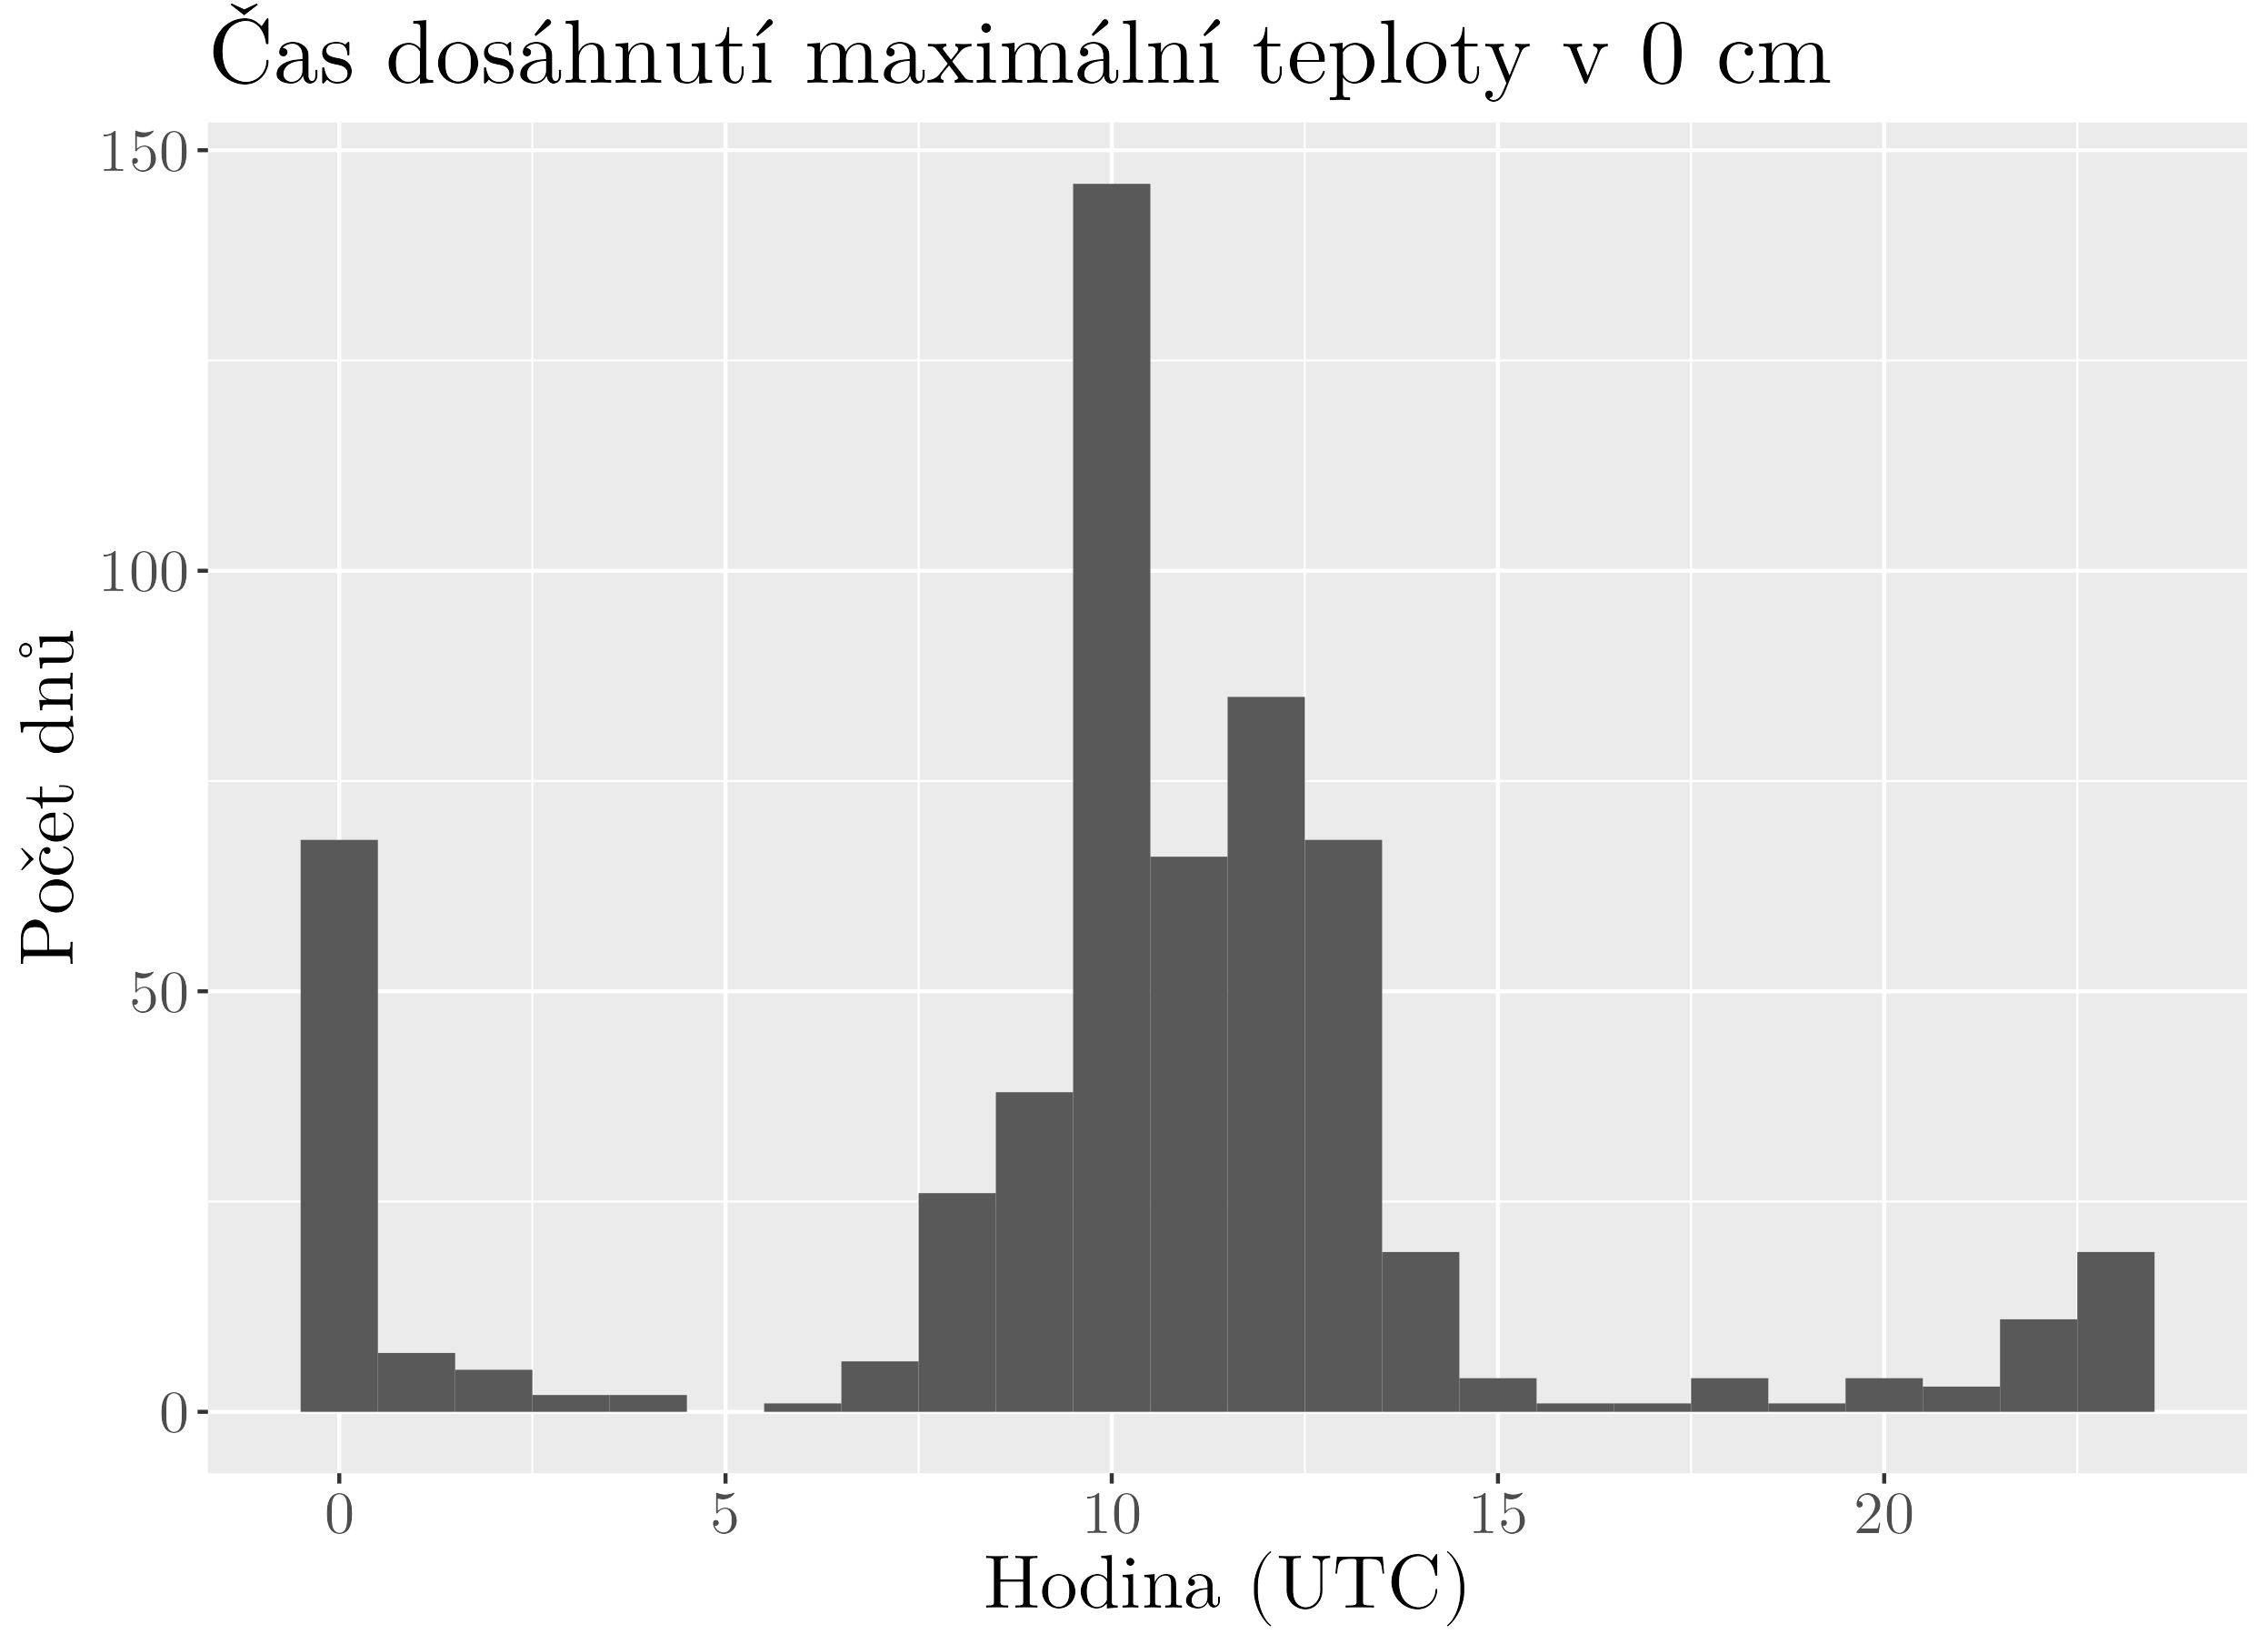
\includegraphics[width=\textwidth]{img/hist_hourmax0cm.png}
		\caption{}
		\label{fig:hourmax0cm}
	\end{subfigure}
	\hfill
	\begin{subfigure}{0.45\textwidth}
  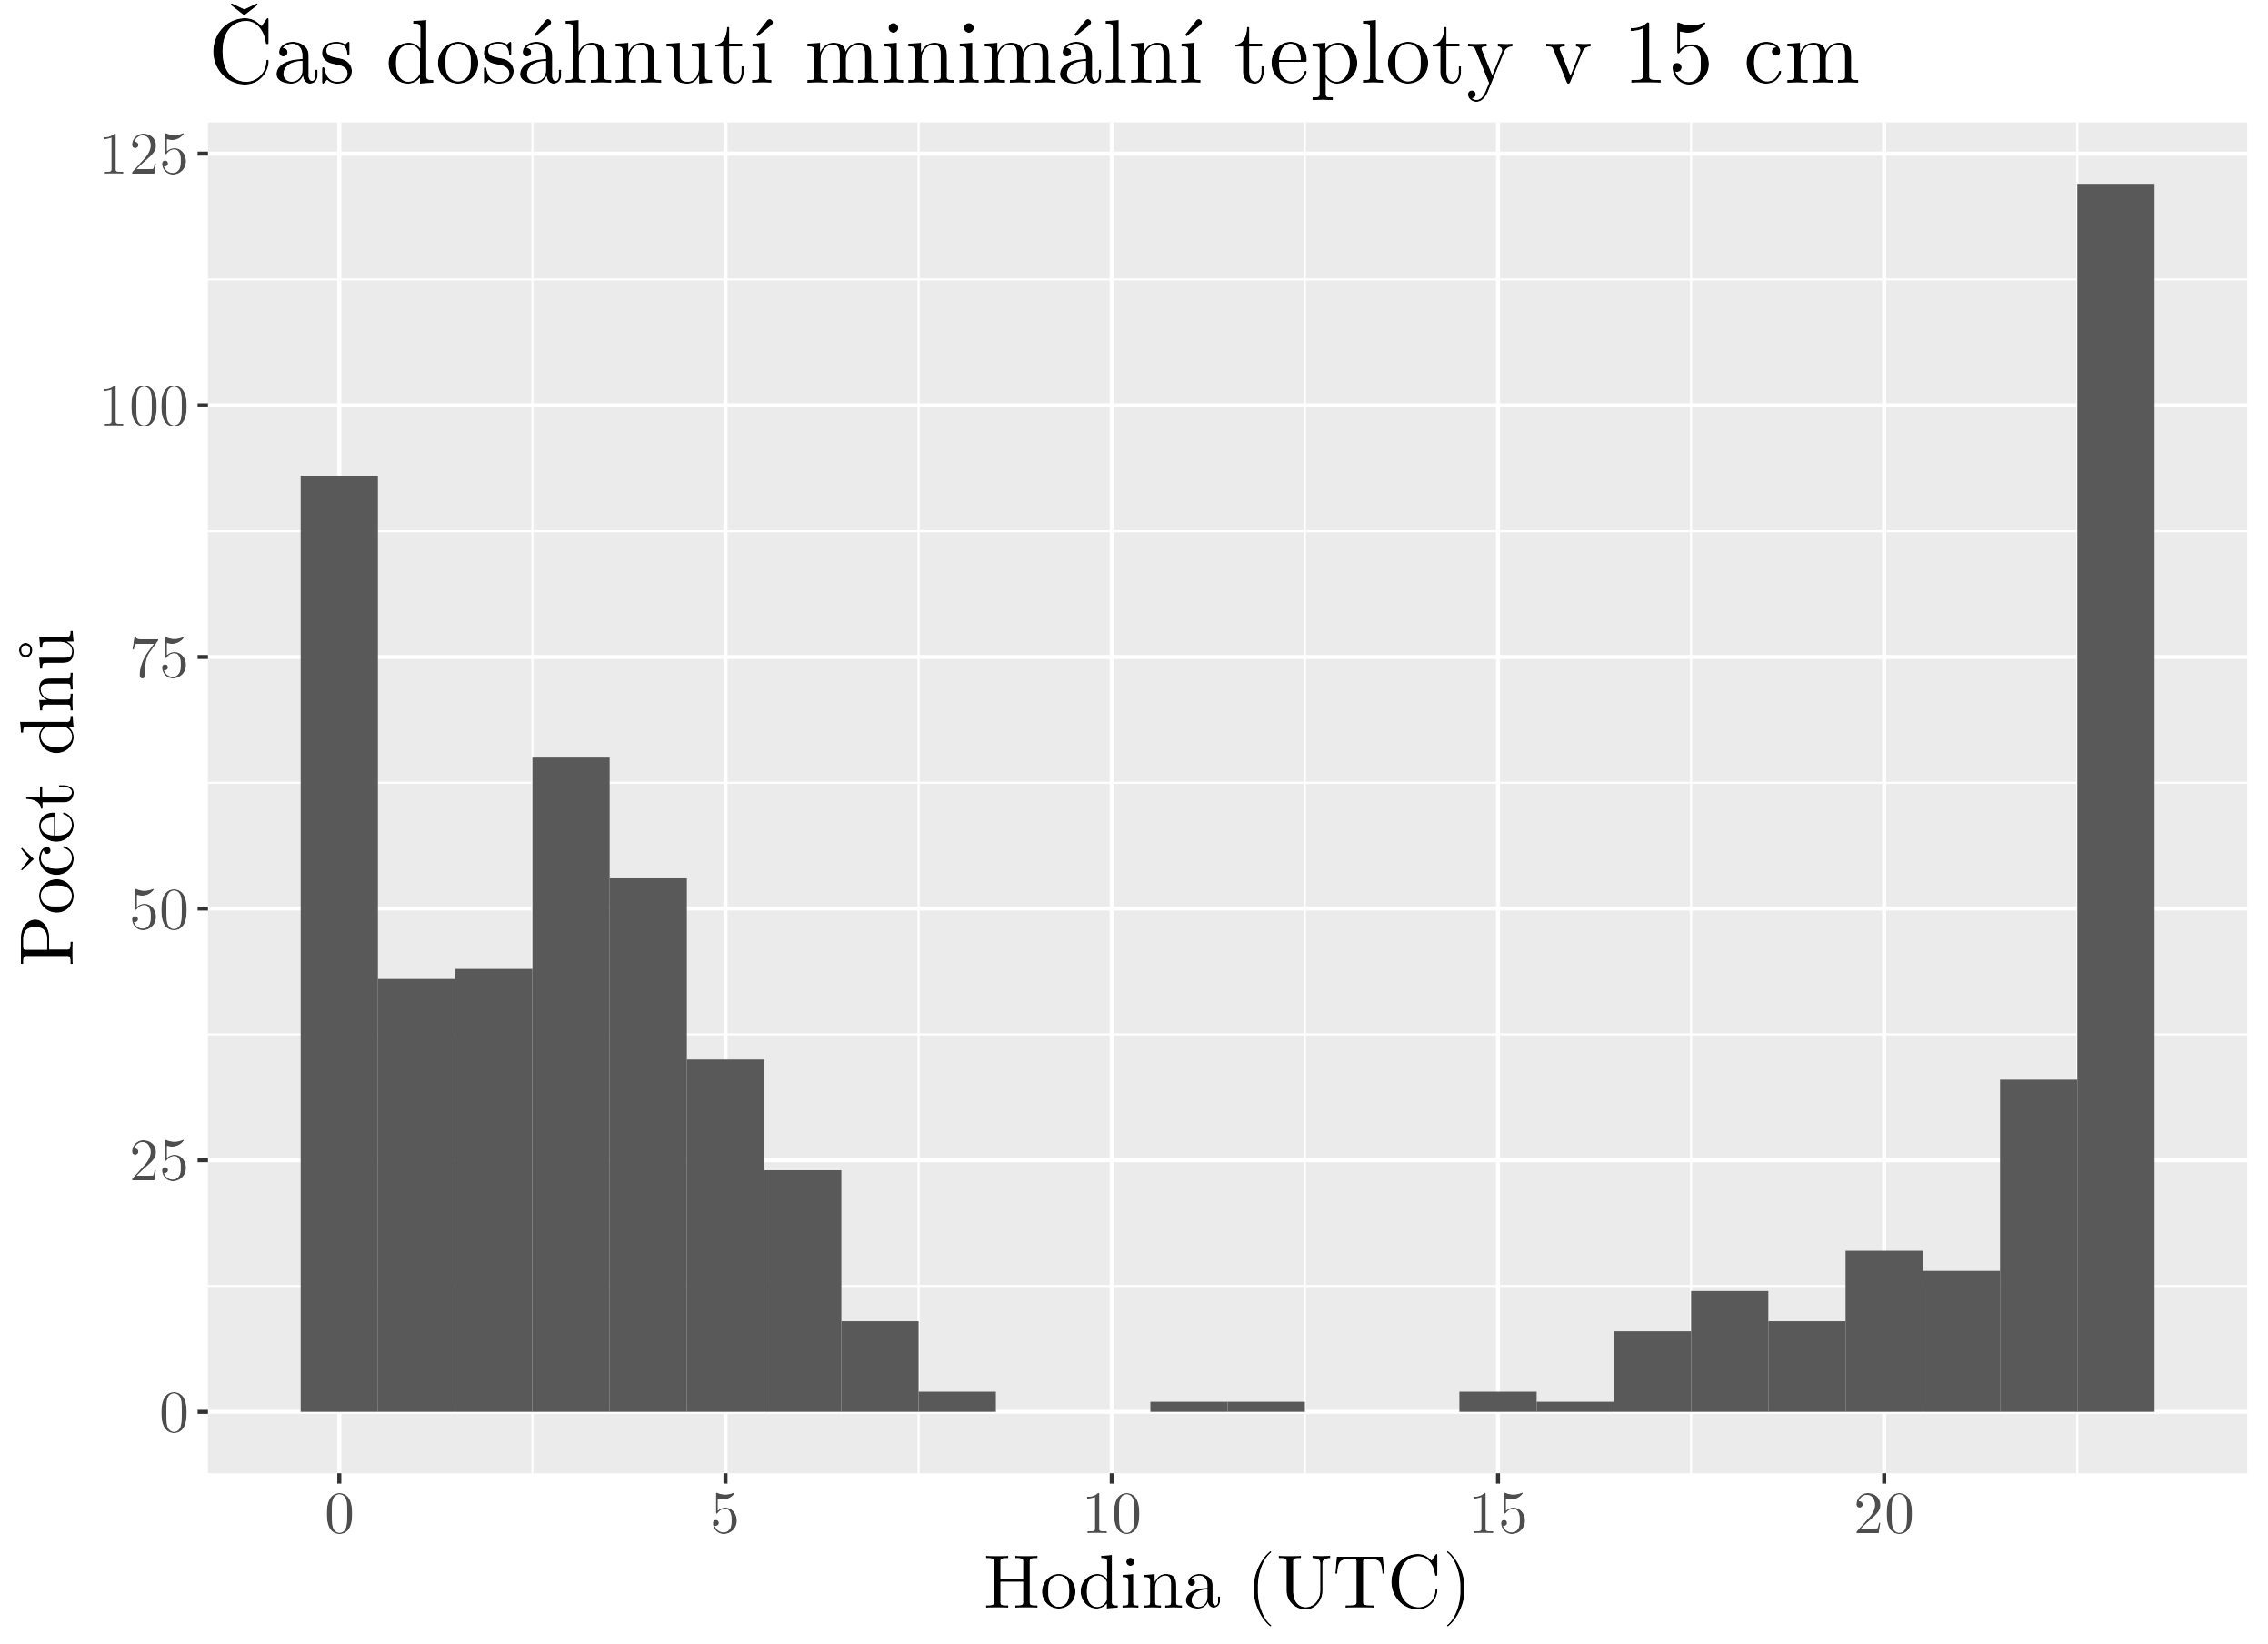
\includegraphics[width=\textwidth]{img/hist_hourmin15cm.png}
		\caption{}
		\label{fig:hourmin15cm}
	\end{subfigure}
	\hfill
	\begin{subfigure}{0.45\textwidth}
  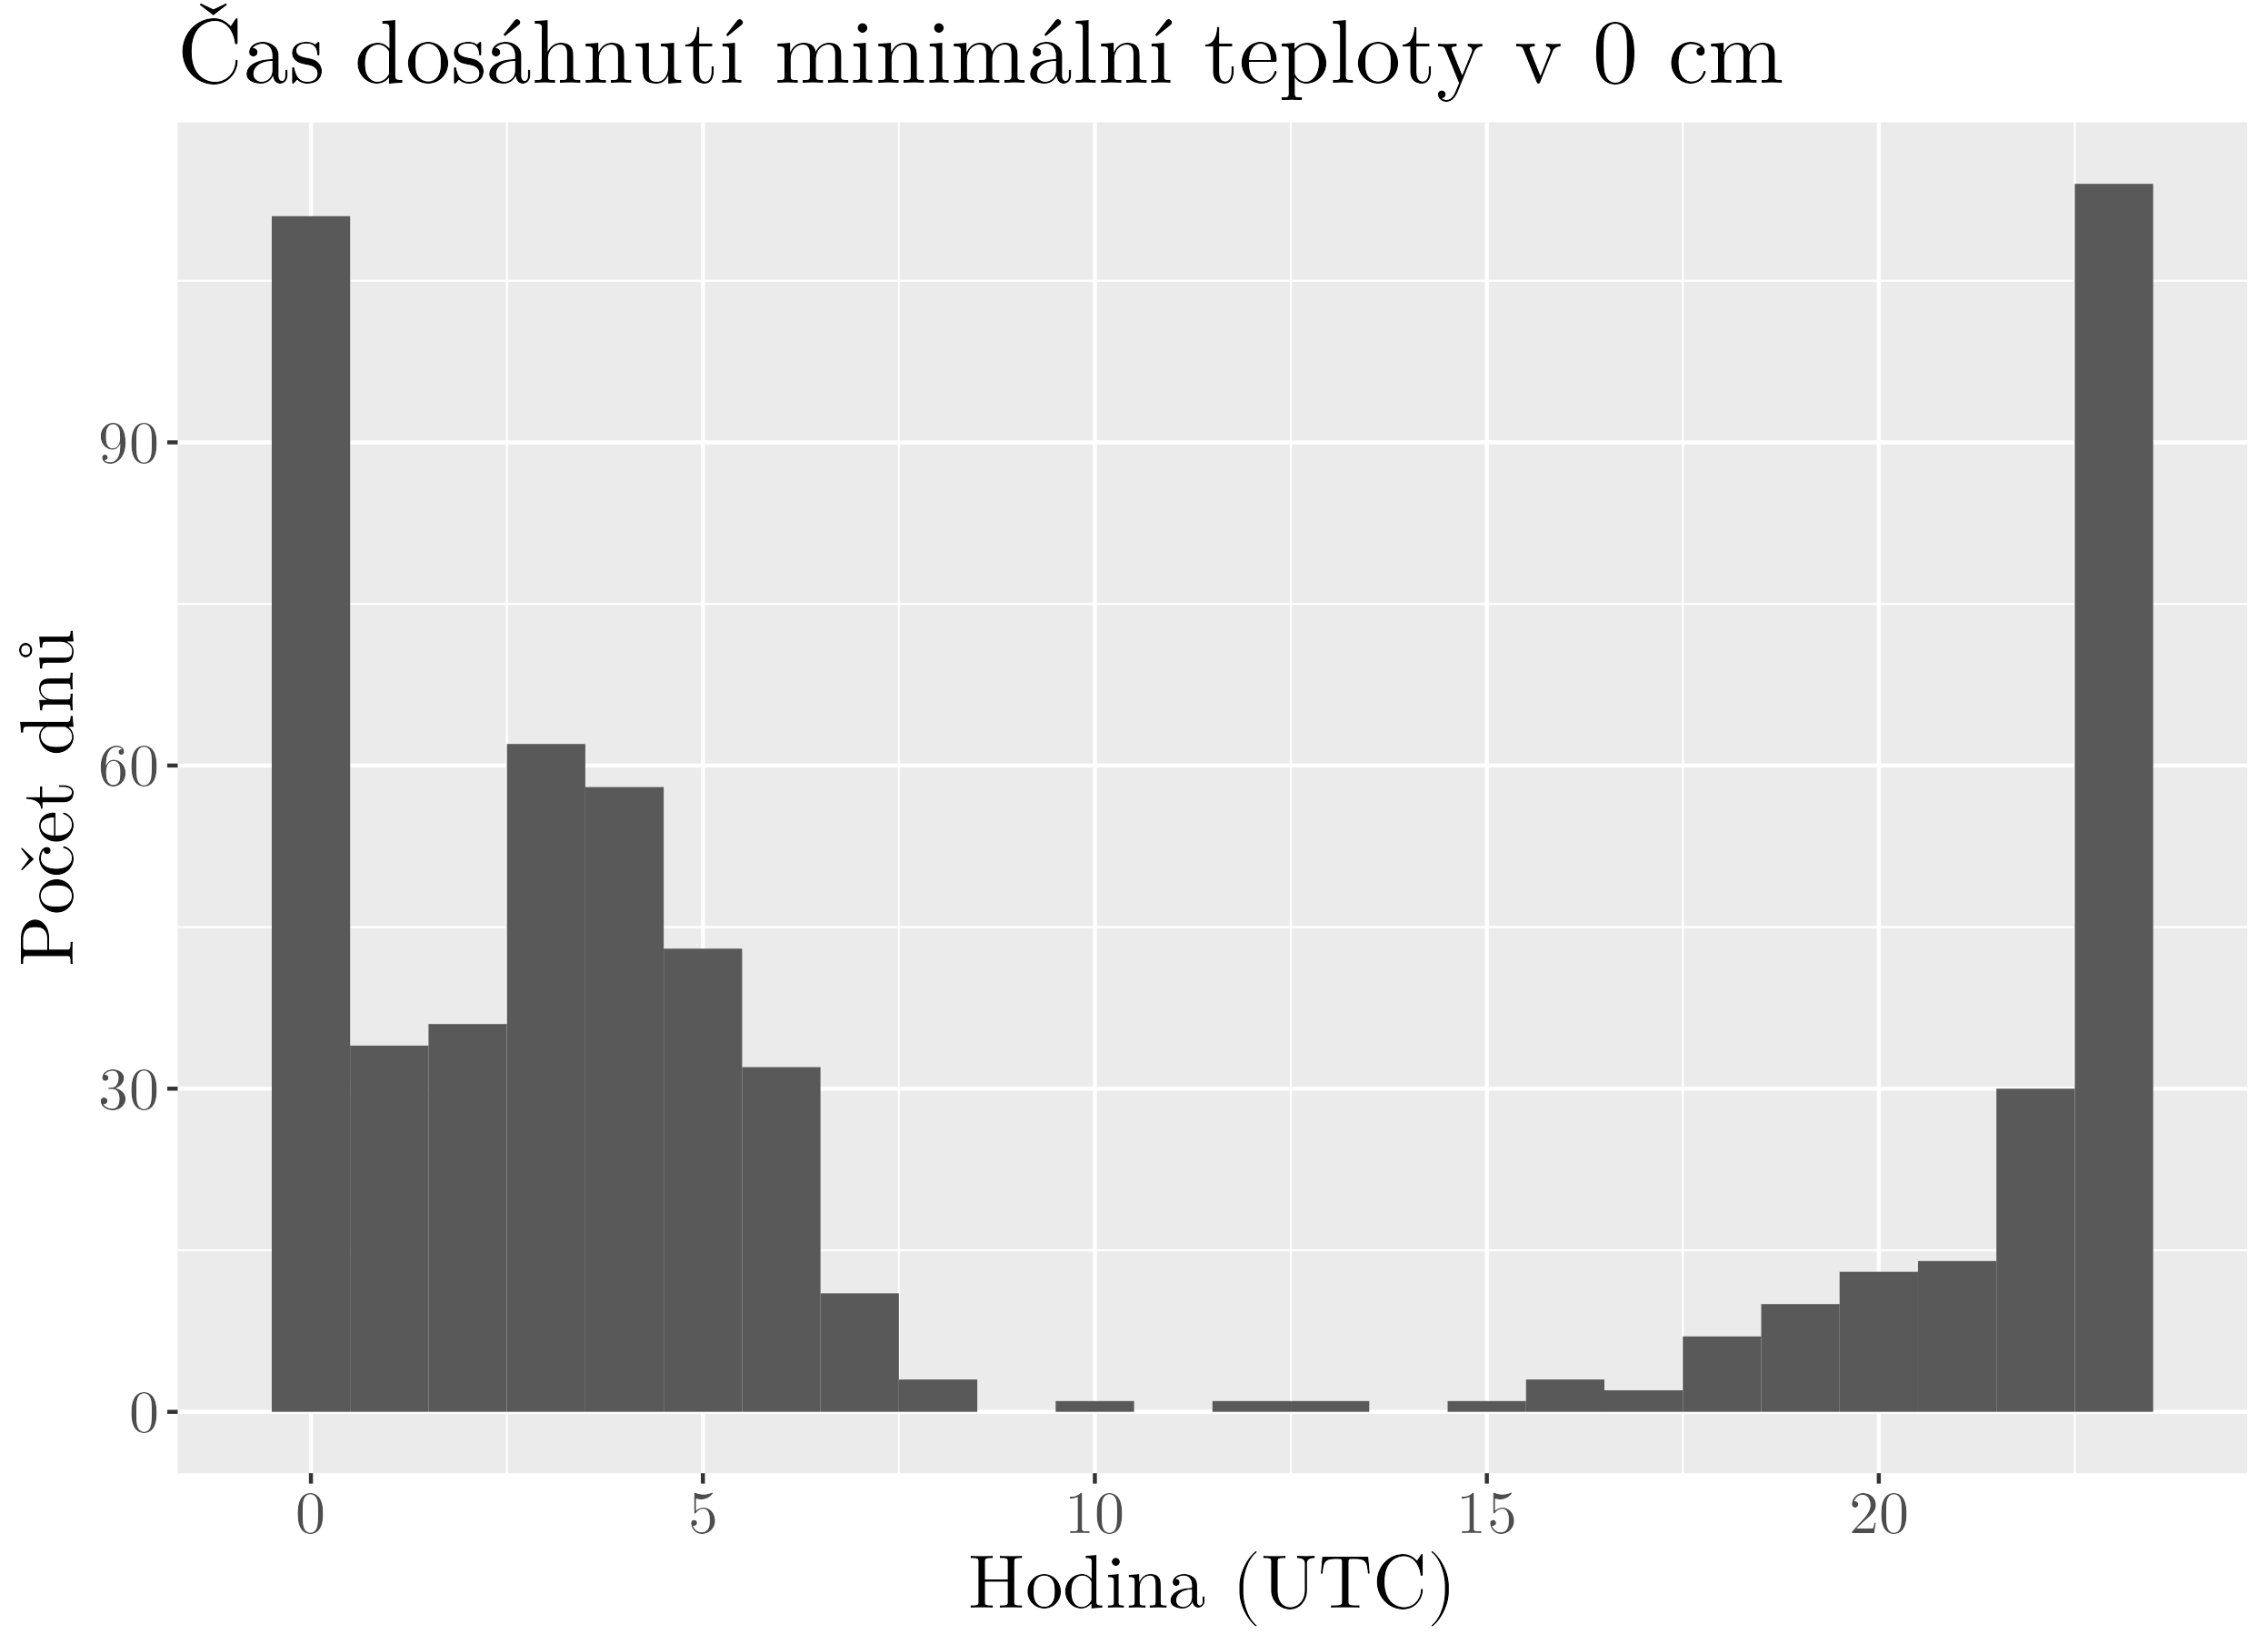
\includegraphics[width=\textwidth]{img/hist_hourmin0cm.png}
		\caption{}
		\label{fig:hourmin0cm}
	\end{subfigure}
	\caption{Denní doba (UTC) dosažení maximální resp. minimální teploty v $\SI{15}{cm}$ resp. v $\SI{0}{cm}$ nad zemí na čidle nejblíže Churáňovu}
	\label{fig:hours}
\end{figure}

Pro ilustraci se ještě podívejme na konkrétní hodnoty teplot pozorované na nejbližším čidlu meteorologické stanice Churáňov. Na obrázcích \ref{fig:hours} můžeme vidět průběh denních minim a maxim na jednom z čidel, celkově jde o období od 12.10.2019 do 20.5.2021 tedy 587 dnů. Na obrázcích \ref{fig:2mhours} můžeme vidět obrázkům \ref{fig:hourmax15cm} a \ref{fig:hourmin15cm} odpovídající hodnoty teplot naměřených ve výšce $\SI{2}{m}$ na čidle zavěšeném na stromě poblíž pozemním čidlům.

\begin{figure}
	\centering
	\begin{subfigure}{0.45\textwidth}
  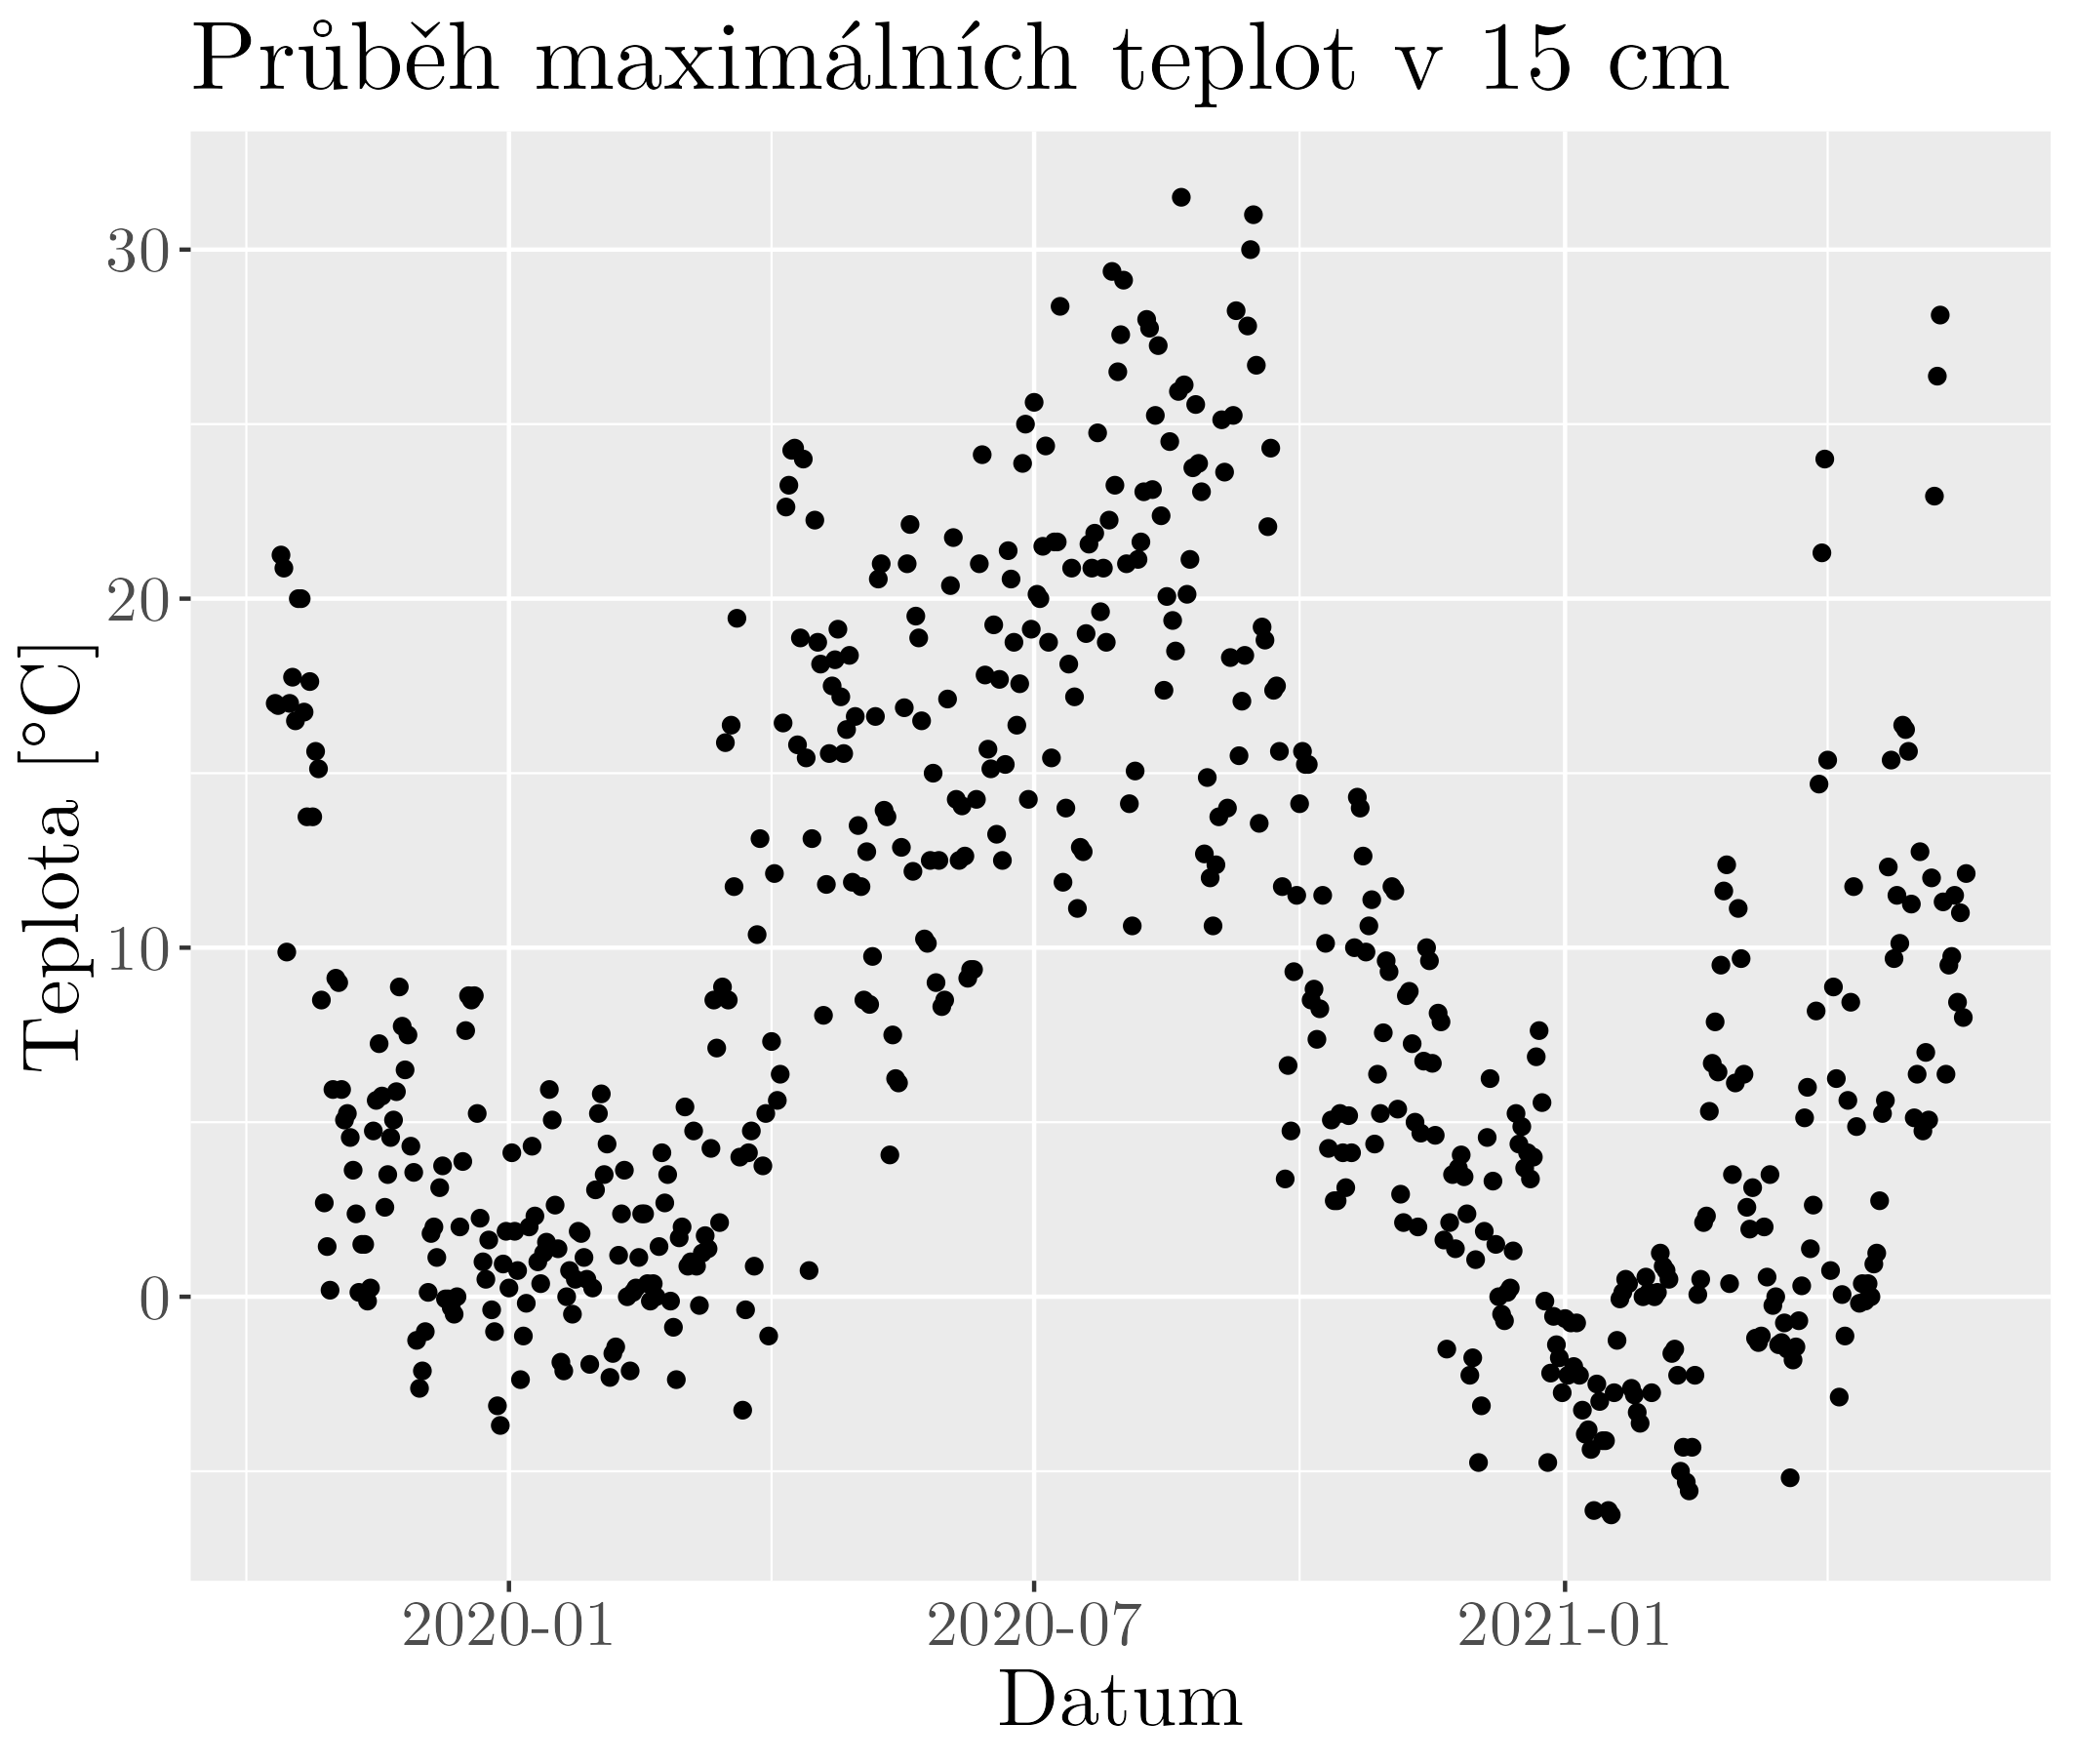
\includegraphics[width=\textwidth]{img/maxtempmax15cm.png}
		\caption{}
		\label{fig:maxtempmax15cm}
	\end{subfigure}
	\hfill
	\begin{subfigure}{0.45\textwidth}
  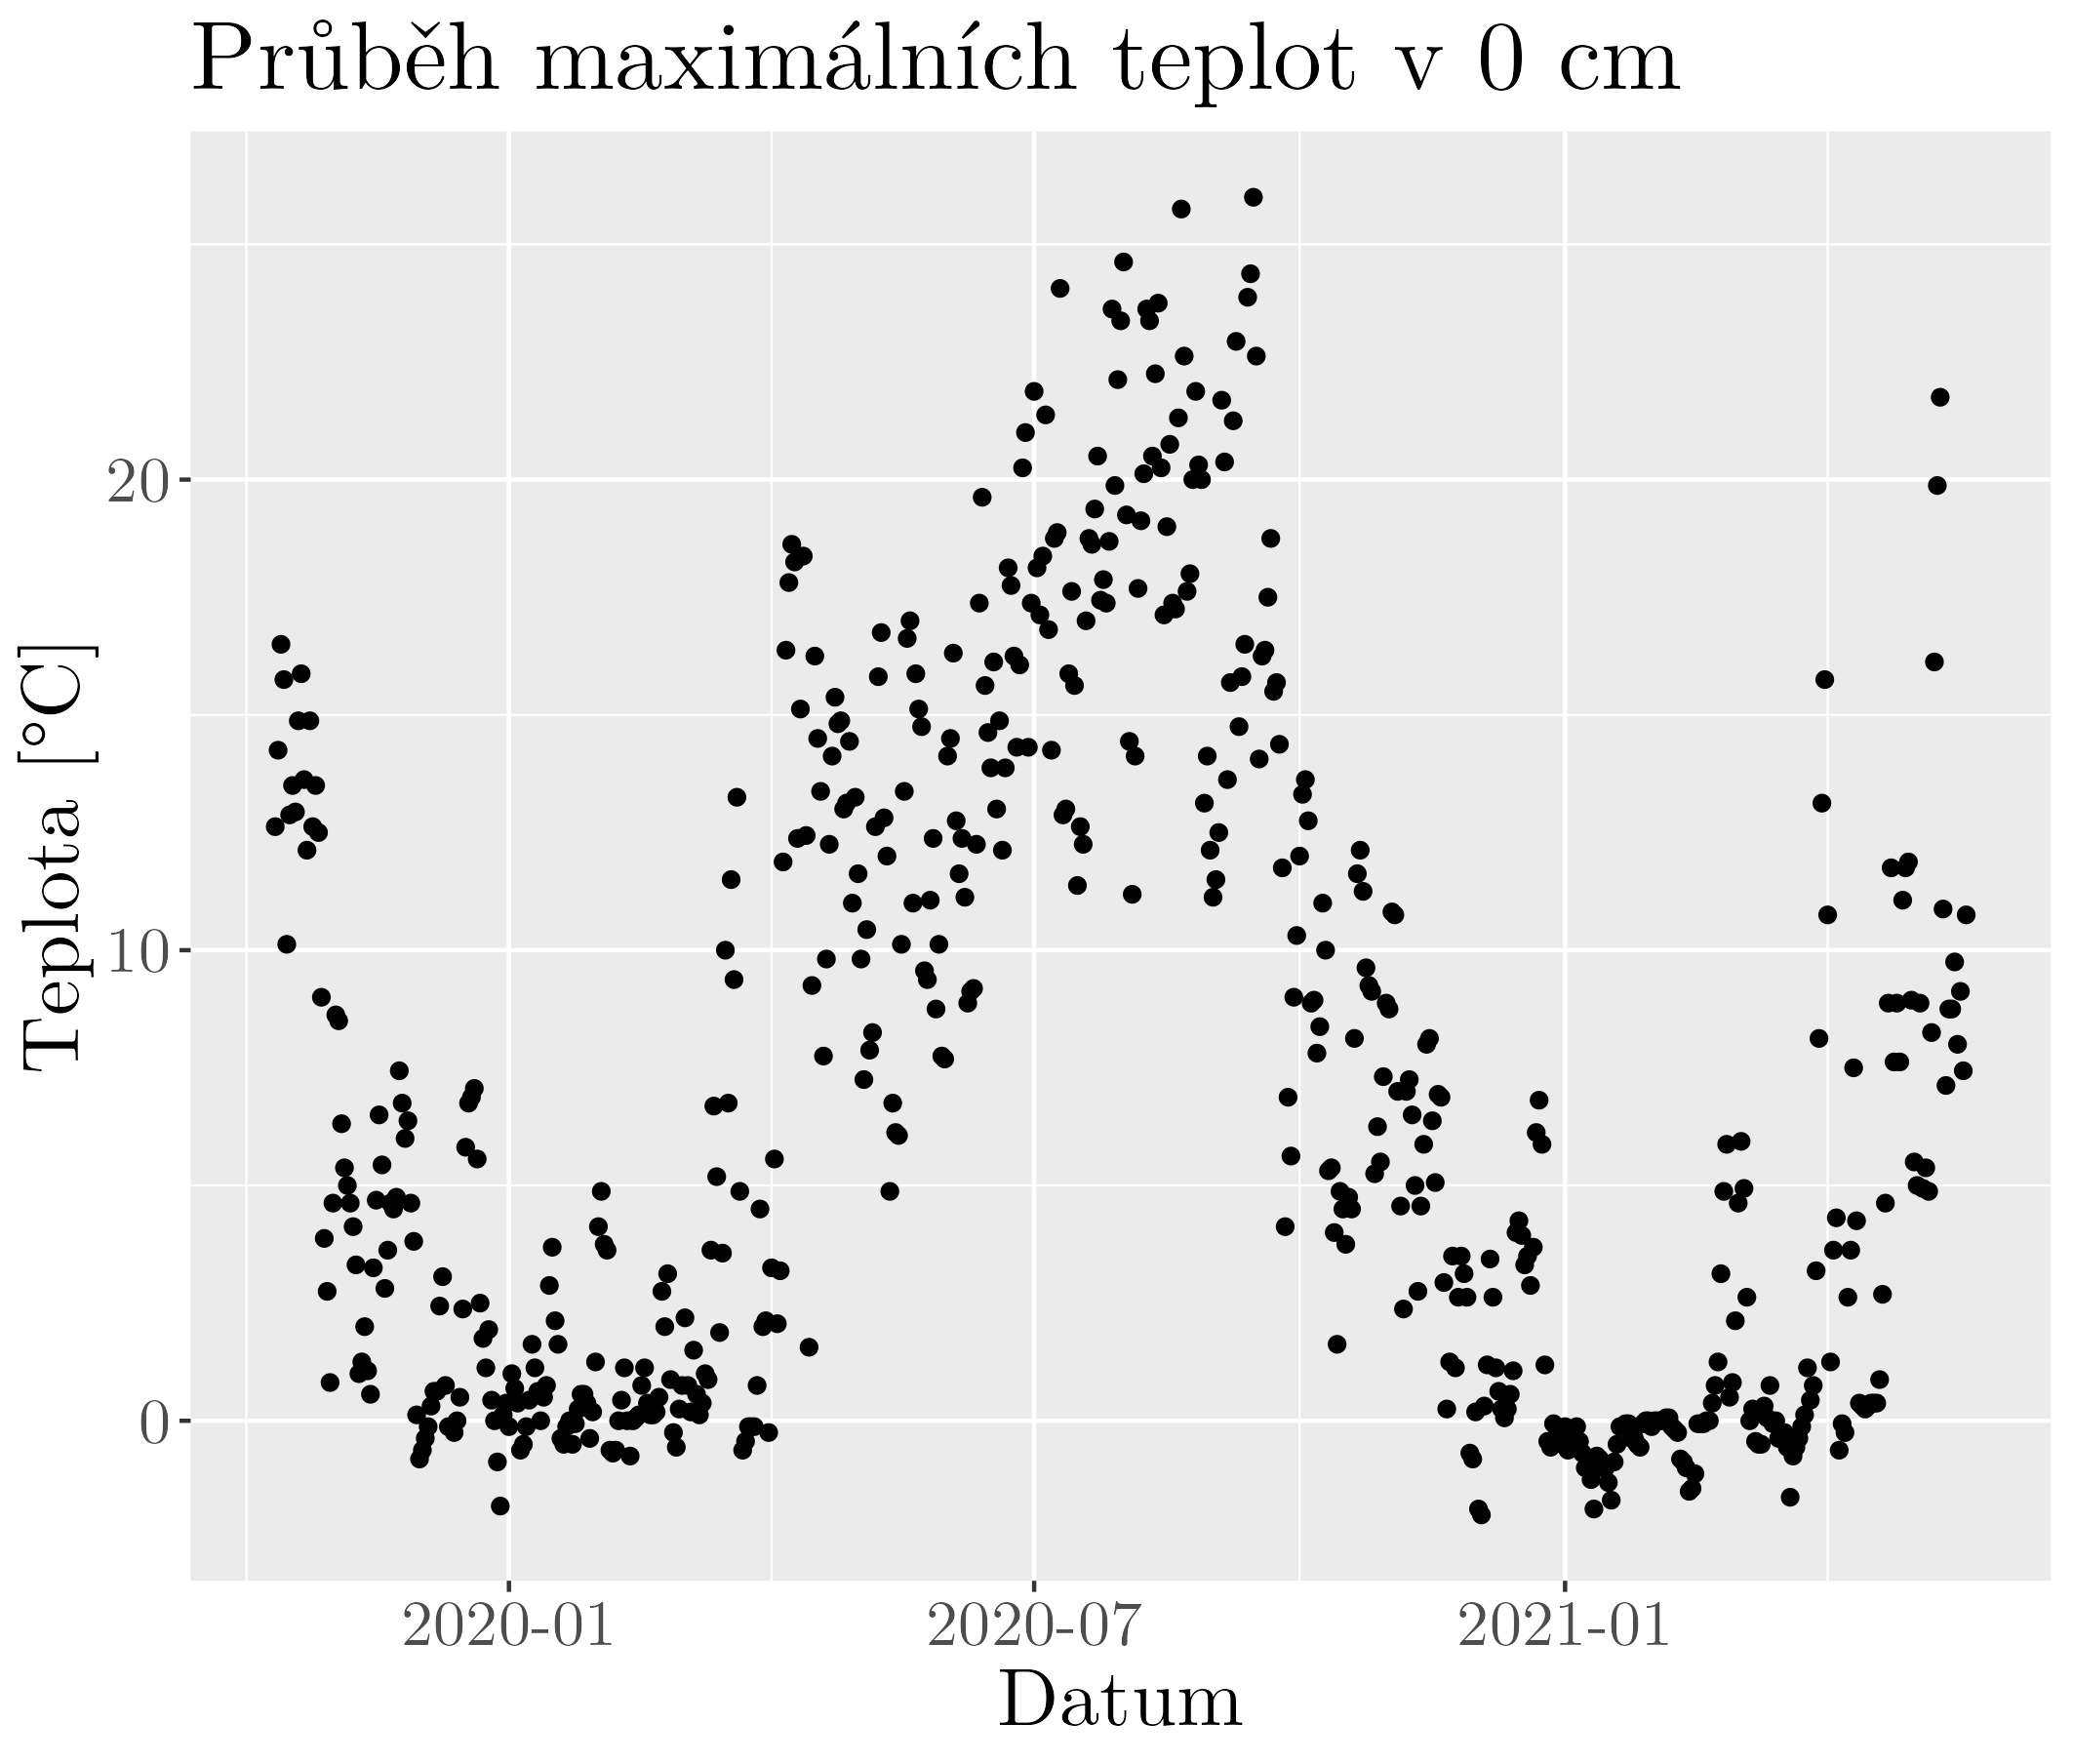
\includegraphics[width=\textwidth]{img/maxtempmax0cm.png}
		\caption{}
		\label{fig:maxtempmax0cm}
	\end{subfigure}
	\hfill
	\begin{subfigure}{0.45\textwidth}
  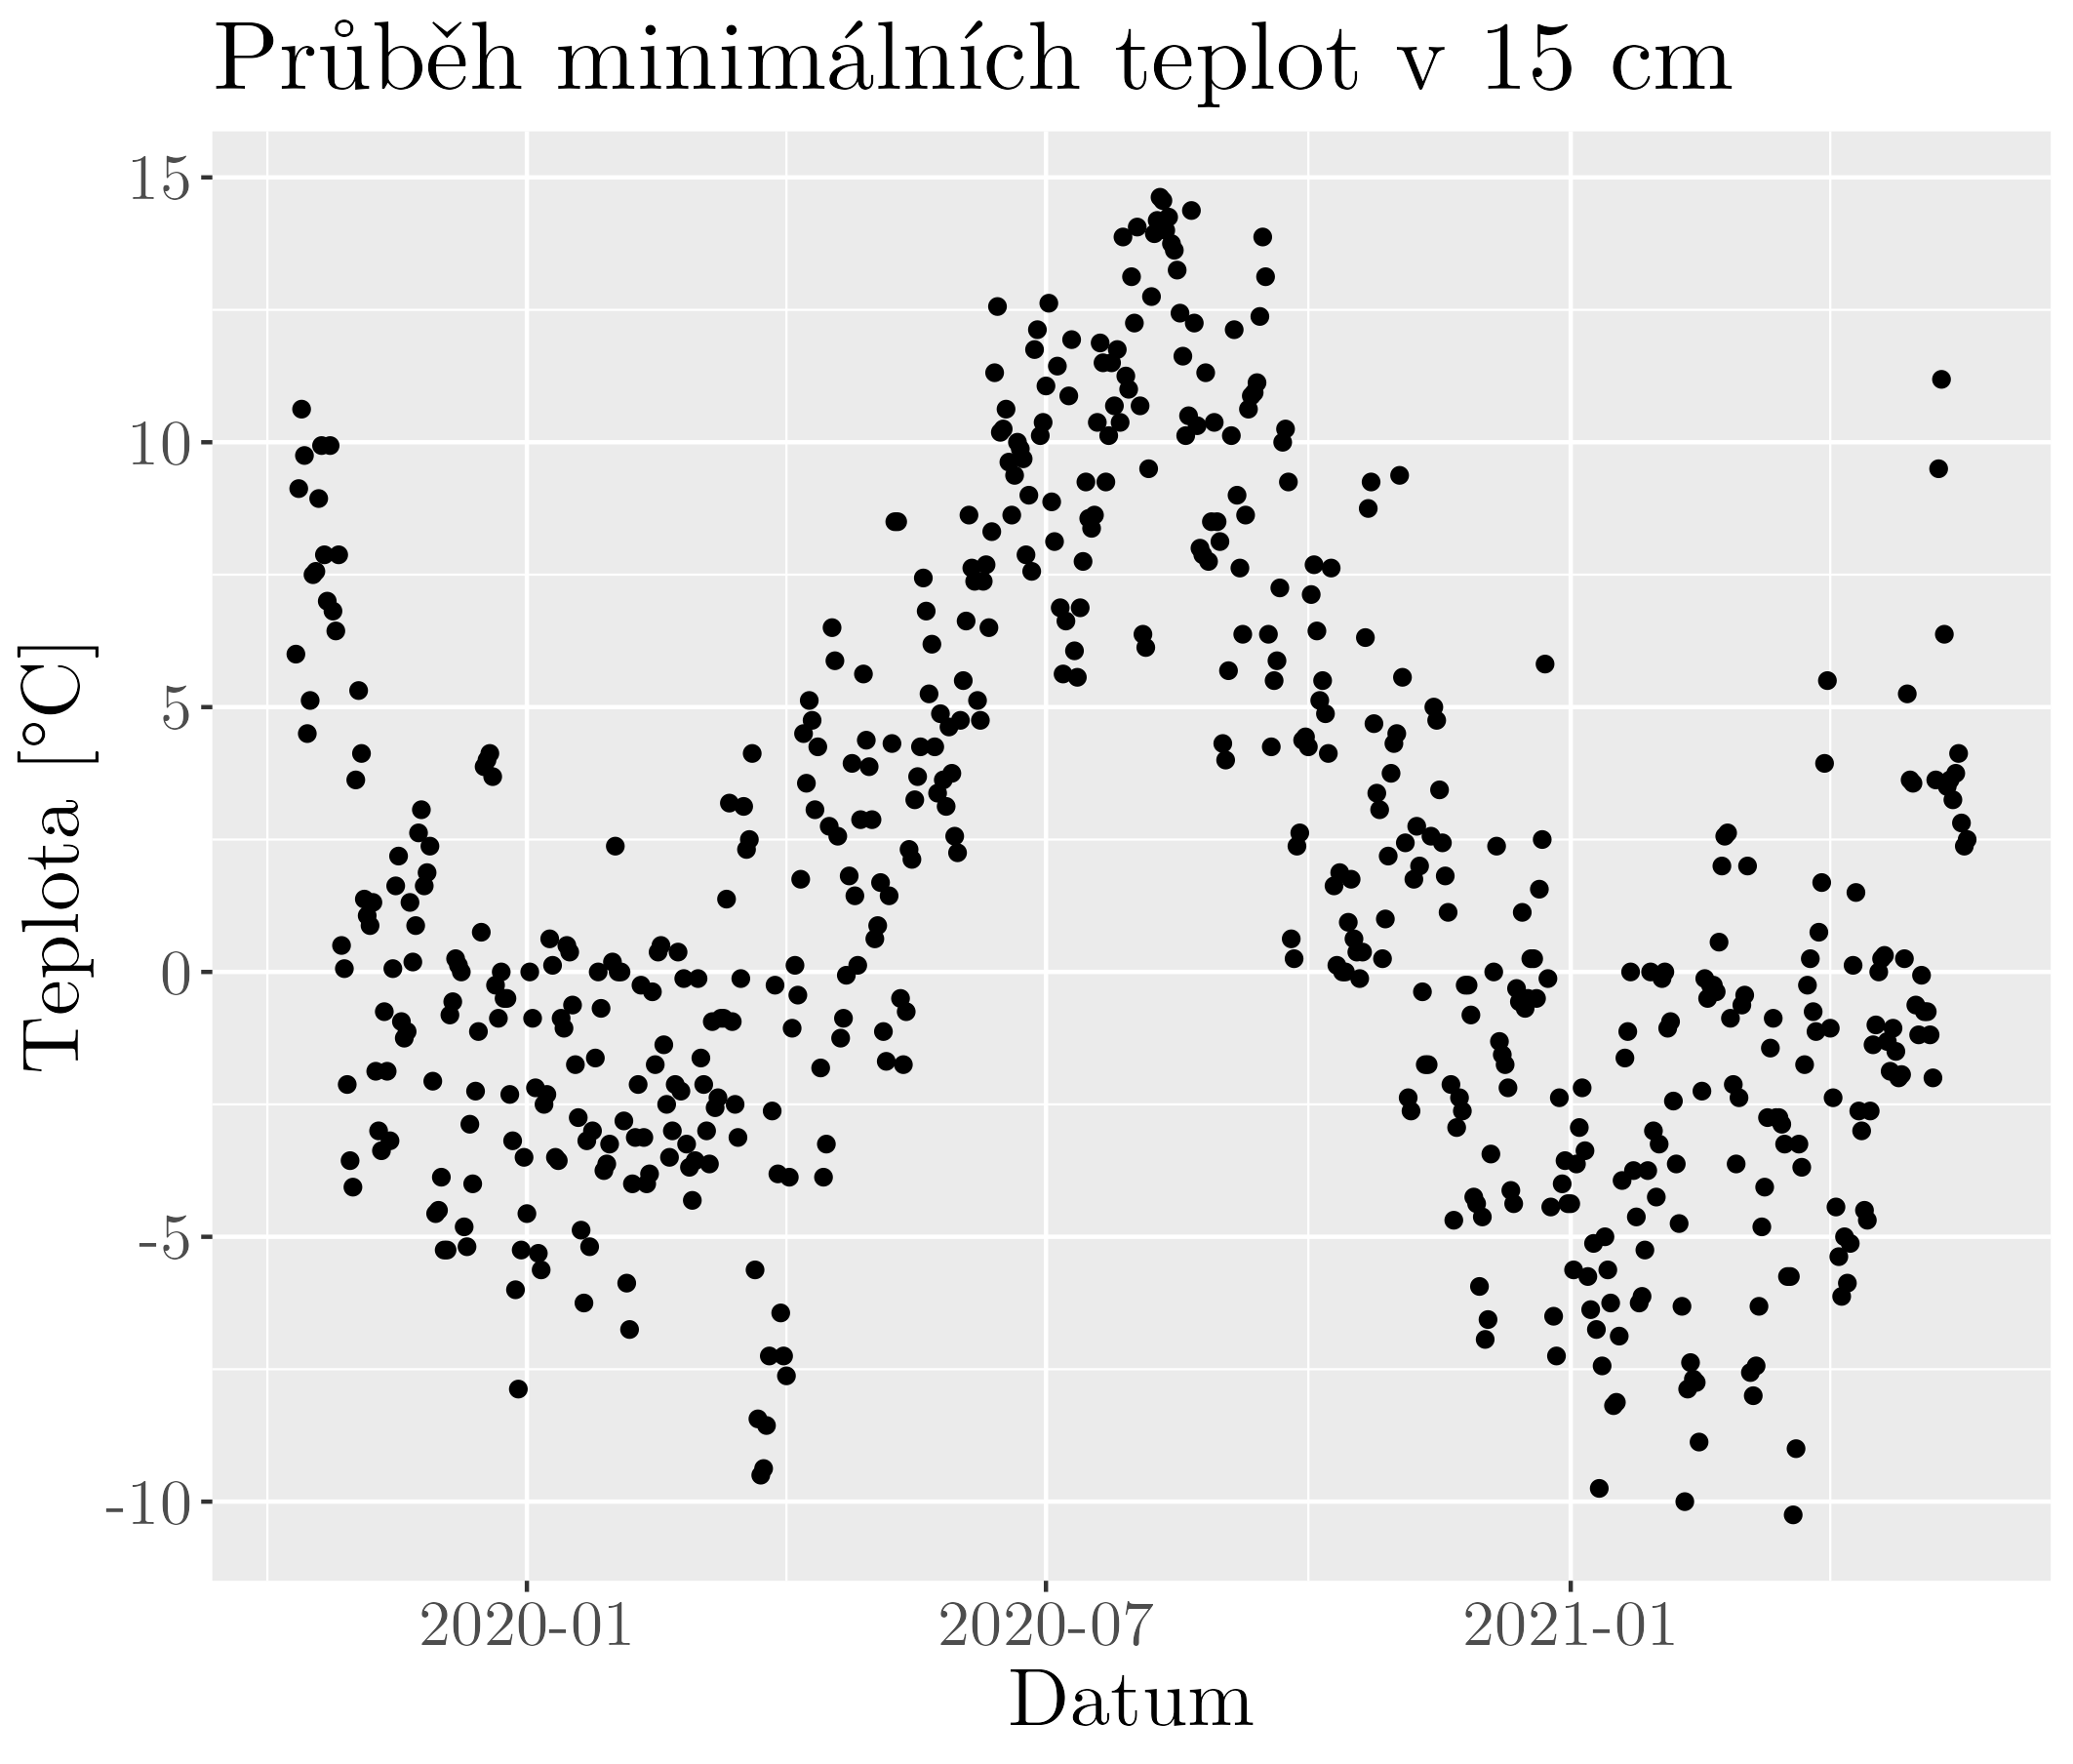
\includegraphics[width=\textwidth]{img/maxtempmin15cm.png}
		\caption{}
		\label{fig:maxtempmin15cm}
	\end{subfigure}
	\hfill
	\begin{subfigure}{0.45\textwidth}
  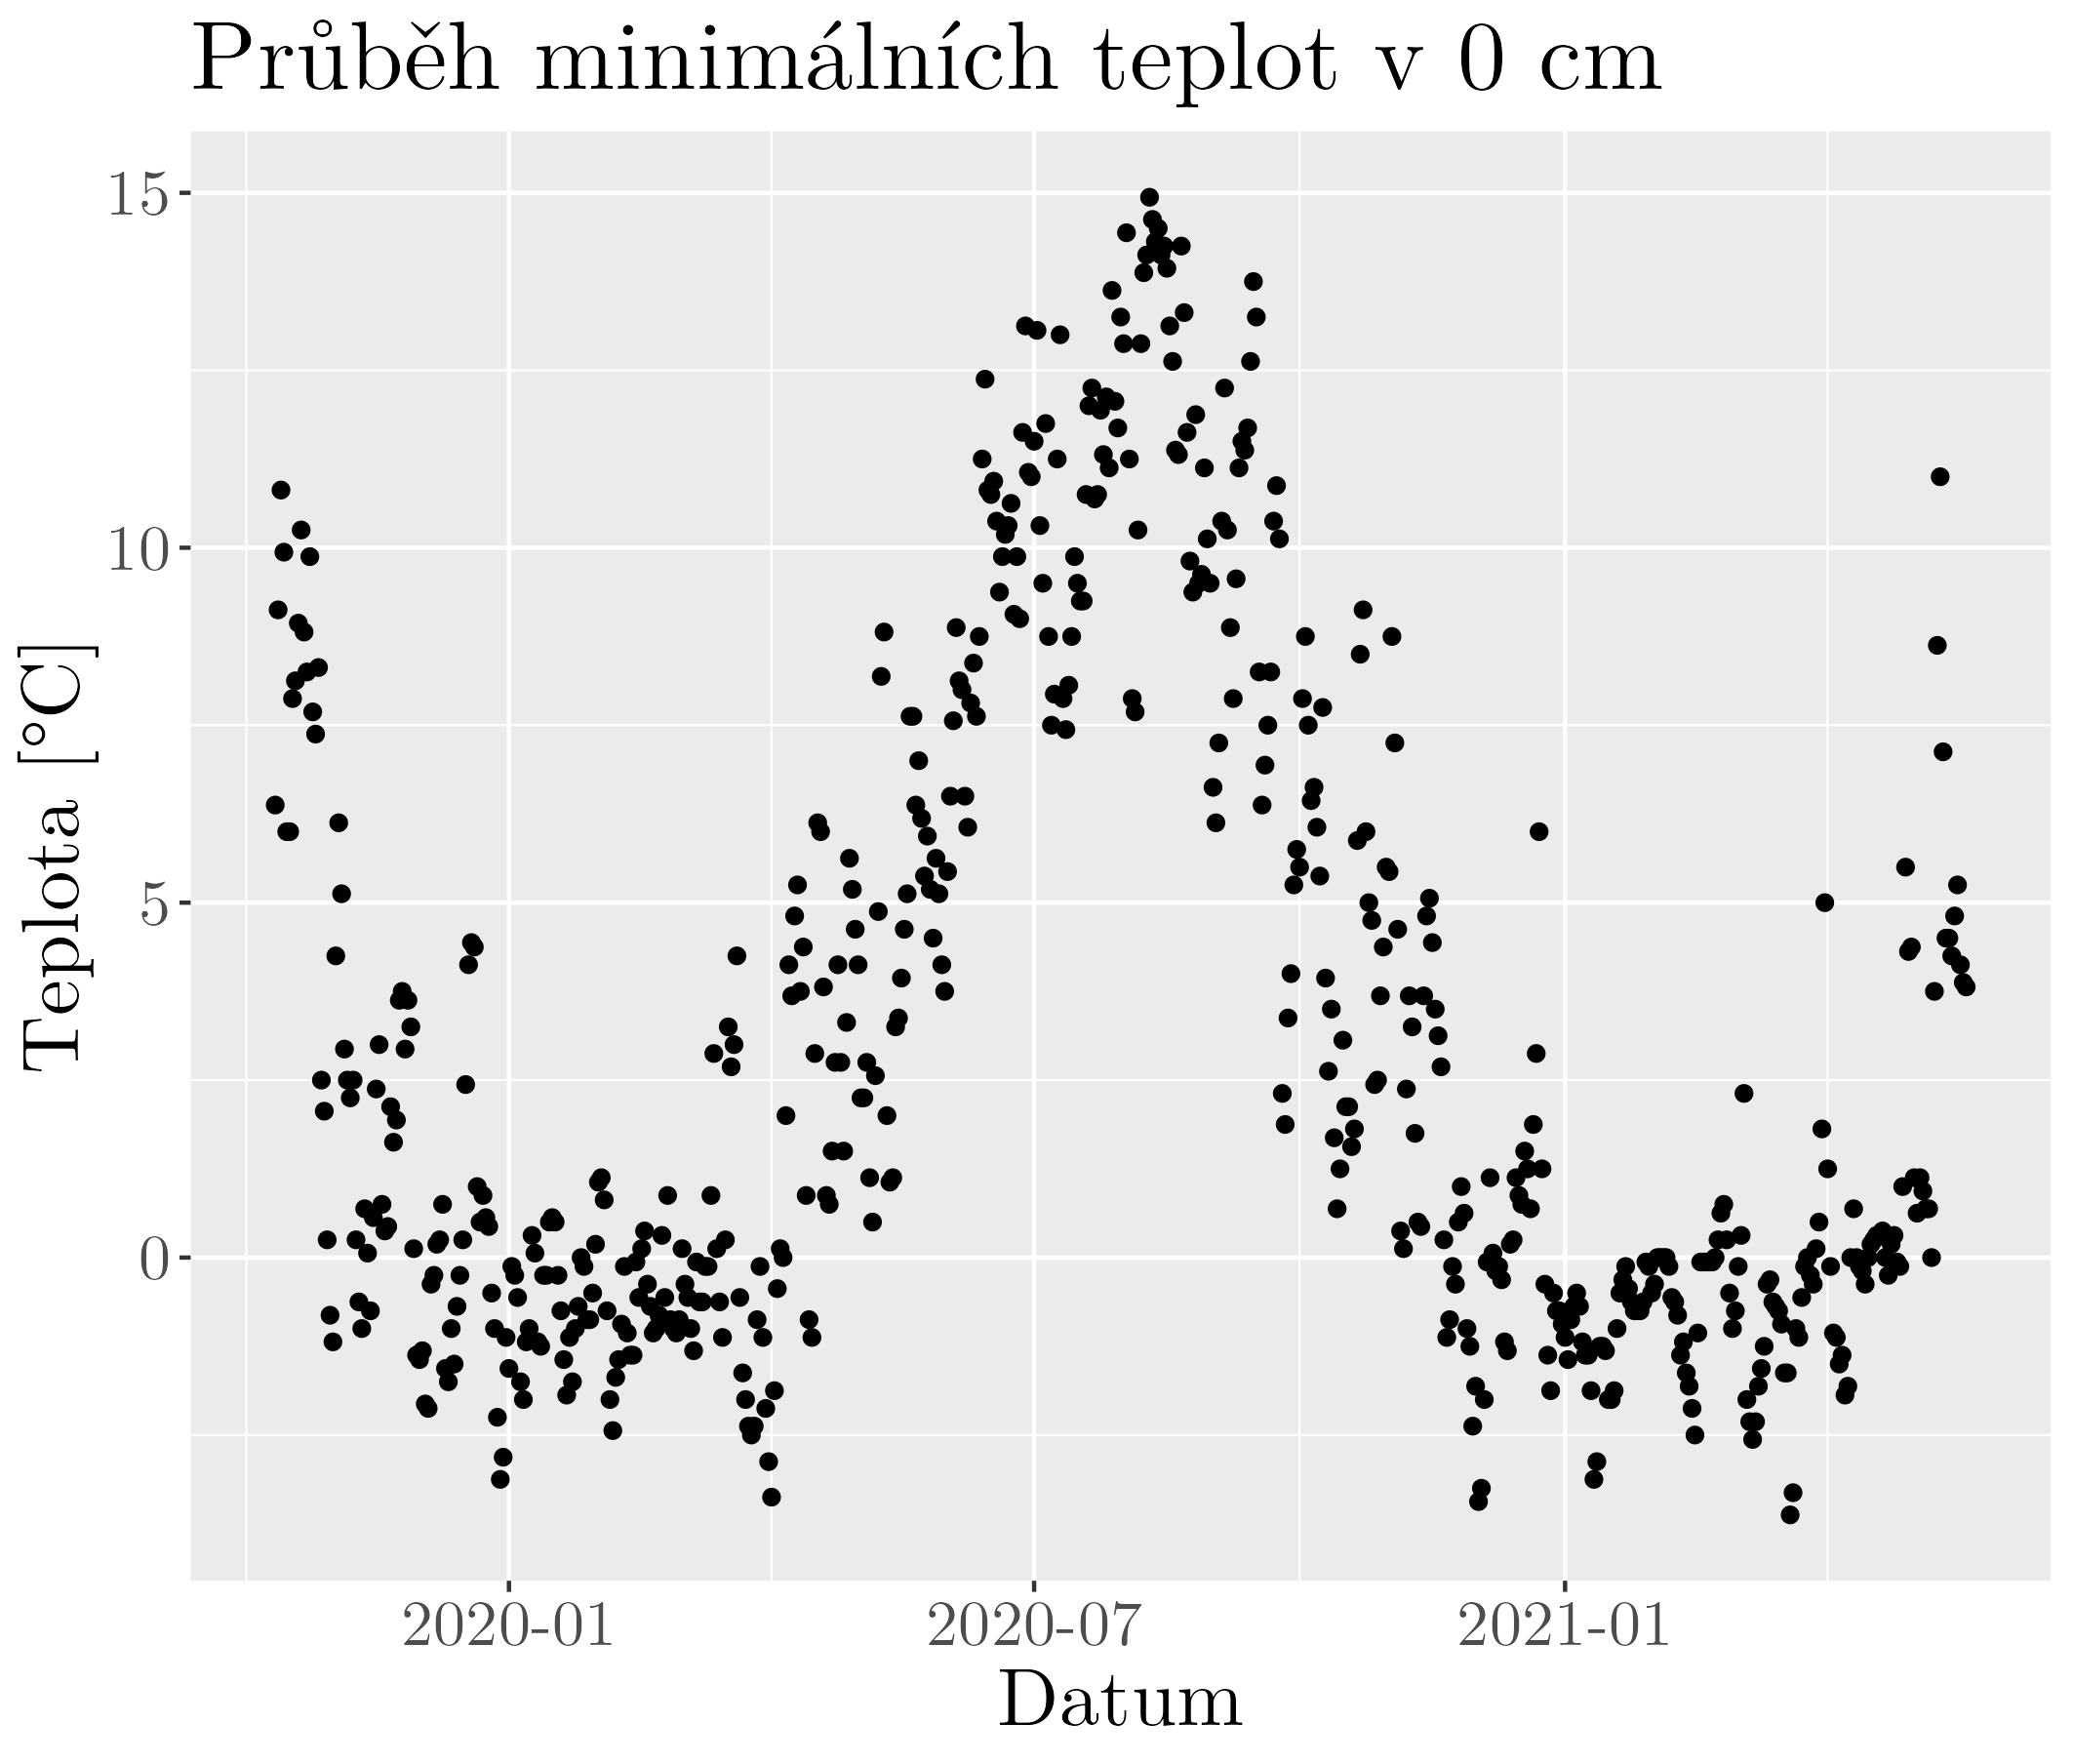
\includegraphics[width=\textwidth]{img/maxtempmin0cm.png}
		\caption{}
		\label{fig:maxtempmin0cm}
	\end{subfigure}
	\caption{Průběh denních maximální resp. minimálních teplot ve výšce $\SI{15}{cm}$ resp. $\SI{0}{cm}$ nad zemí na čidle nejblíže Churáňovu}
	\label{fig:hours}
\end{figure}

\begin{figure}
	\centering
	\begin{subfigure}{0.45\textwidth}
  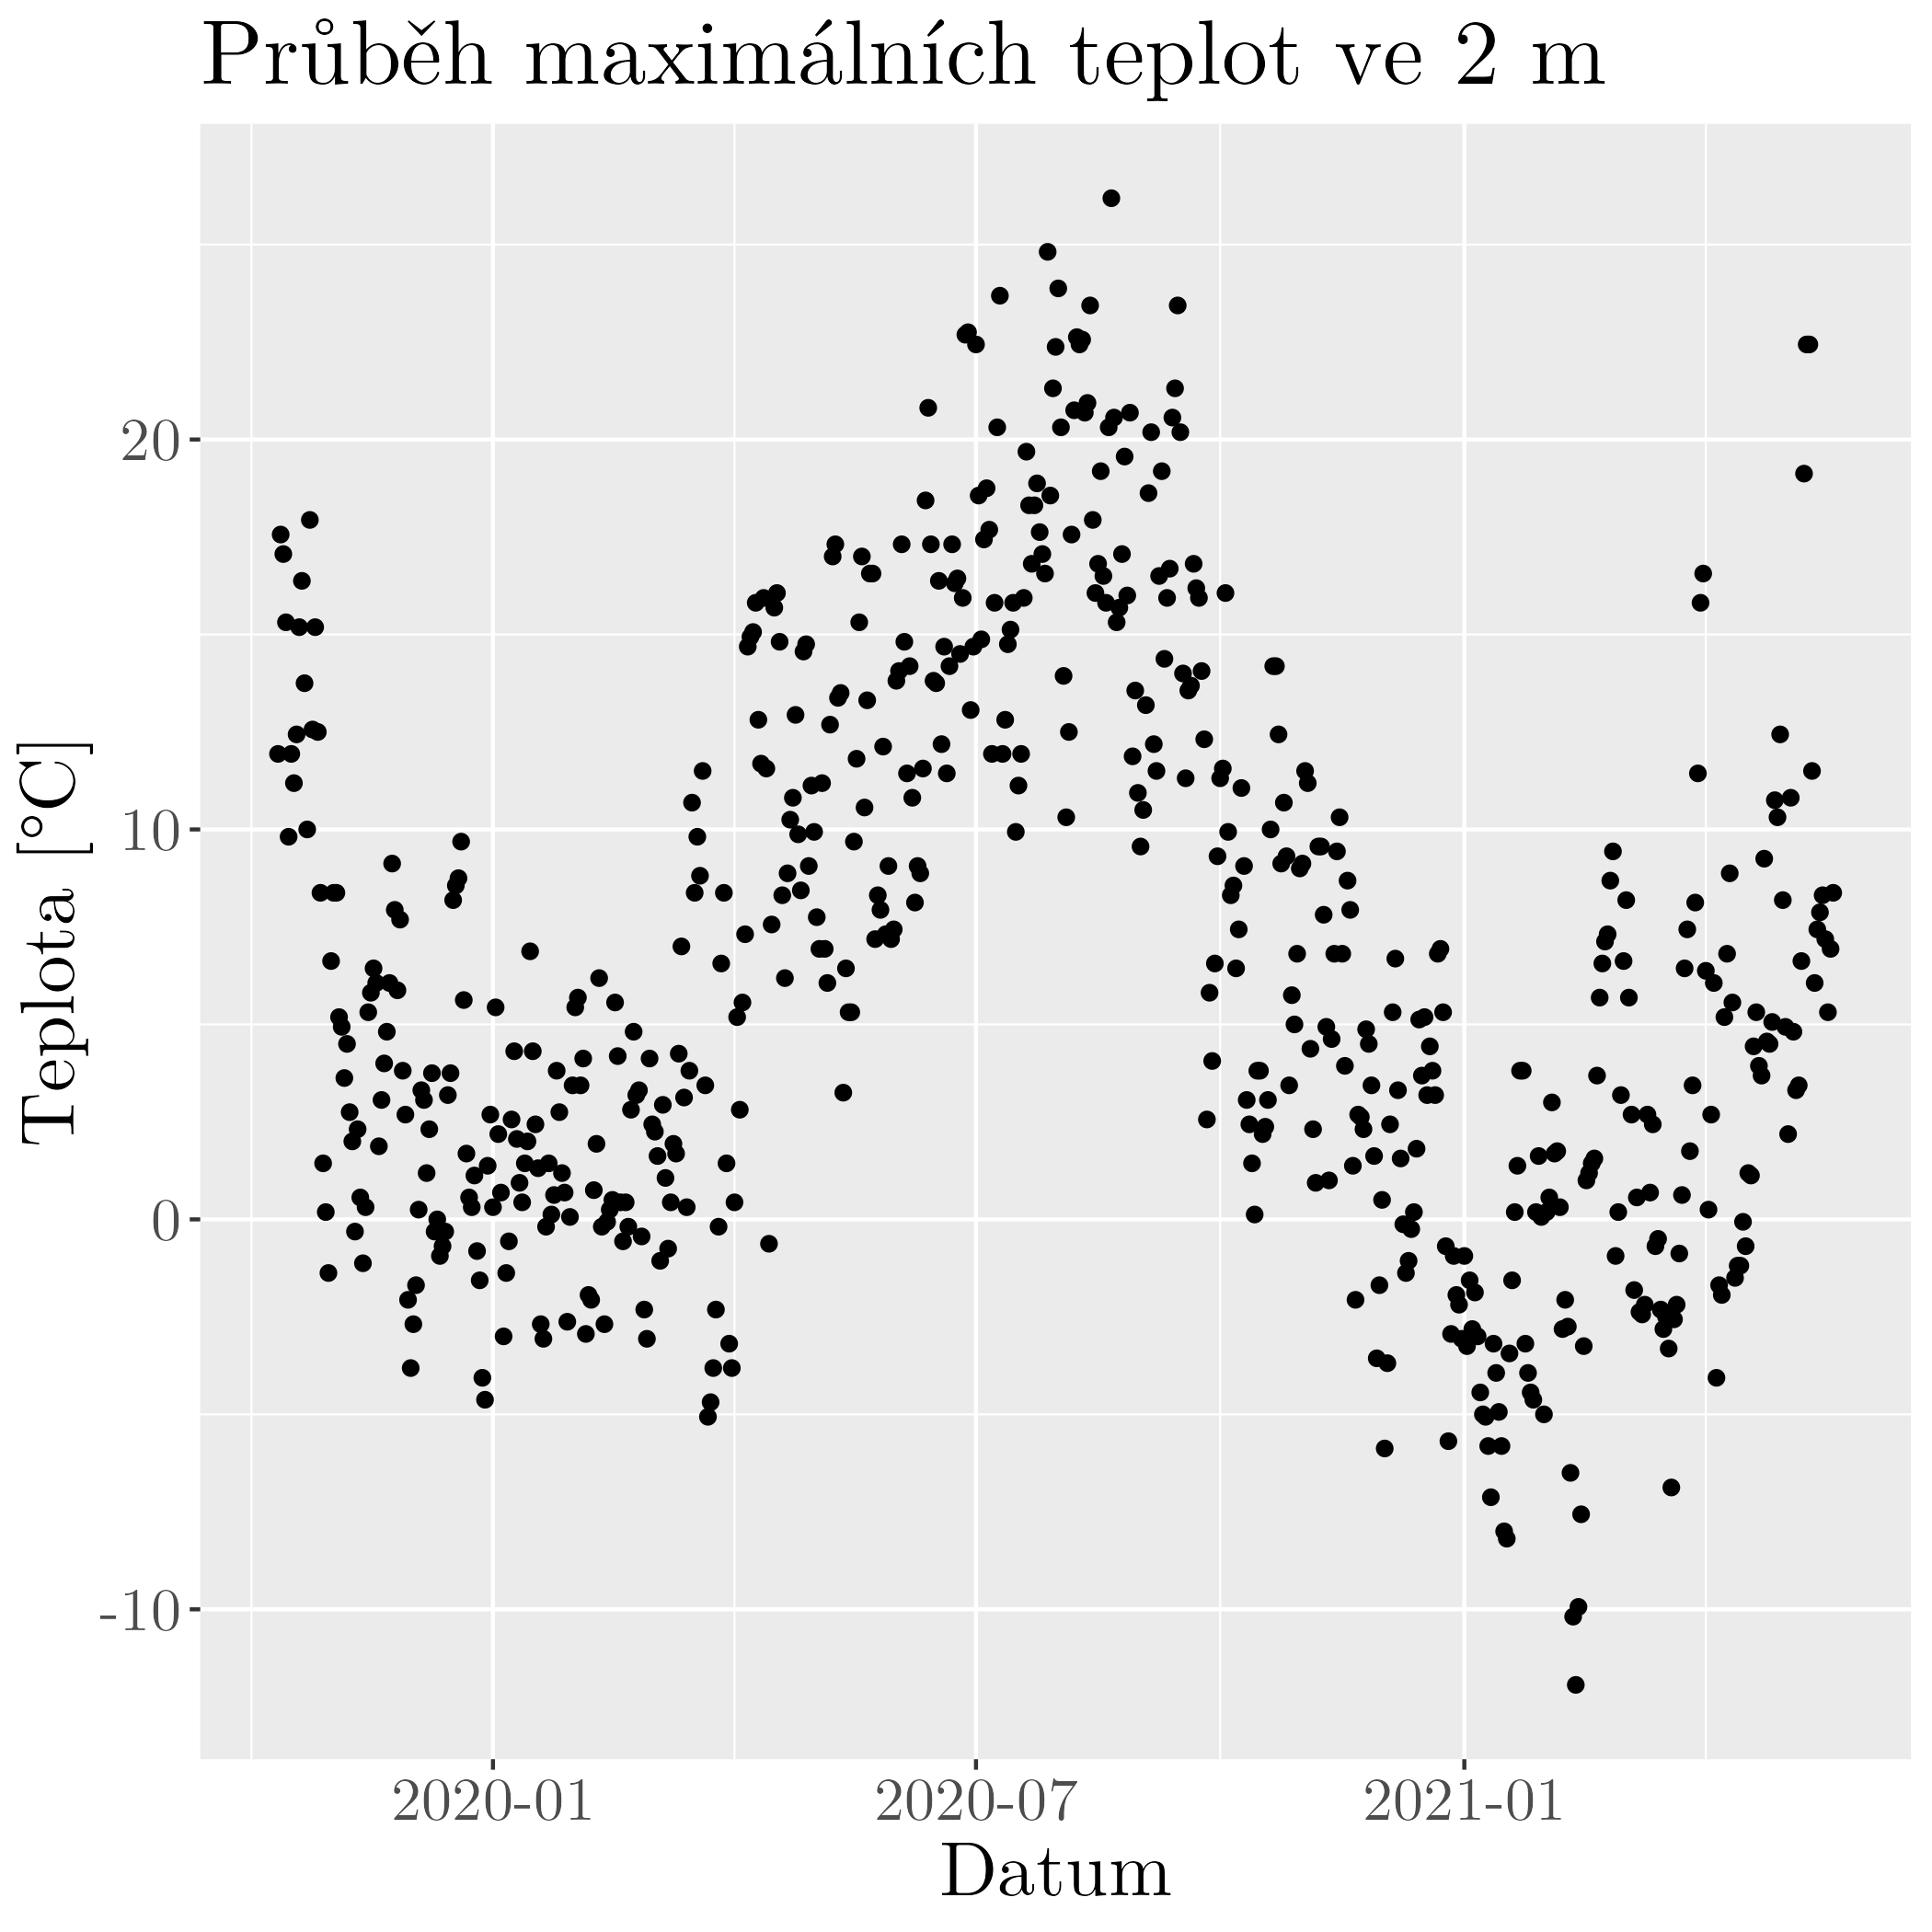
\includegraphics[width=\textwidth]{img/2mmaxtempmax15cm.png}
		\caption{Teploty naměřené ve stejnou dobu jako maximální teploty v $\SI{15}{cm}$}
		\label{fig:2mmaxtempmax15cm}
	\end{subfigure}
	\hfill
	\begin{subfigure}{0.45\textwidth}
  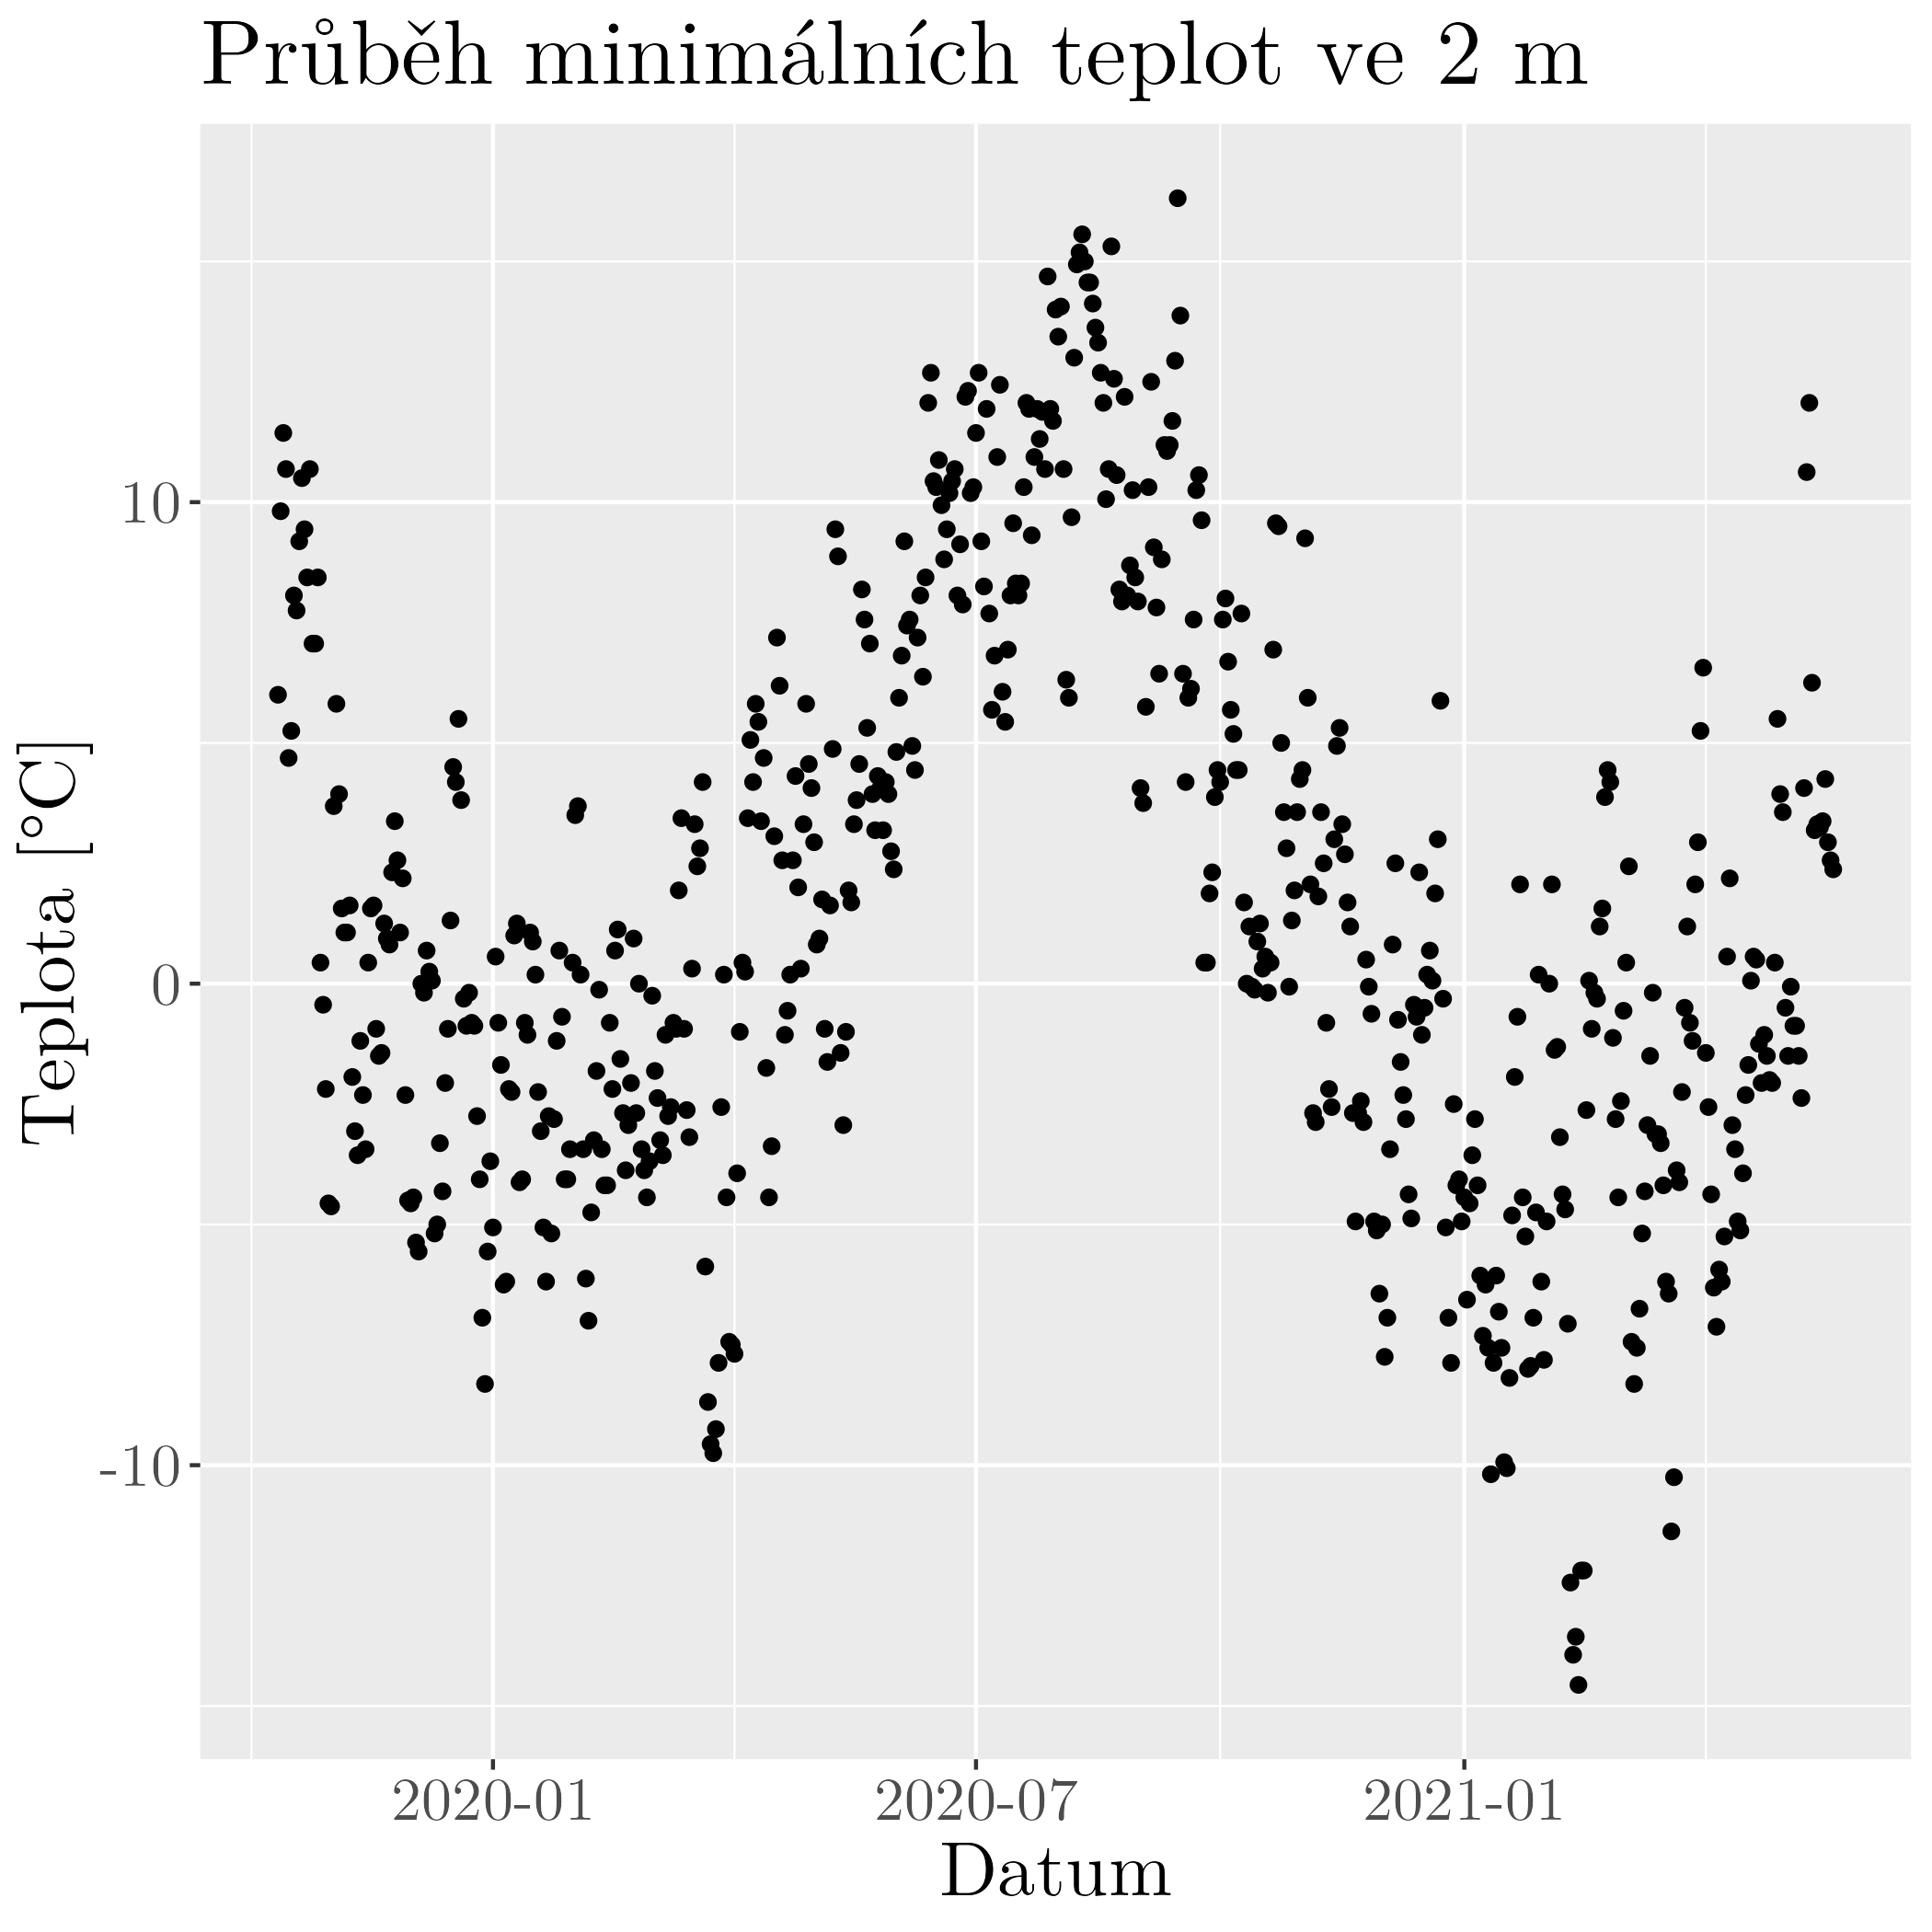
\includegraphics[width=\textwidth]{img/2mmaxtempmin15cm.png}
		\caption{Teploty naměřené ve stejnou dobu jako minimální teploty v $\SI{15}{cm}$}
		\label{fig:2mmaxtempmin15cm}
	\end{subfigure}
	\caption{Teploty ve výšce $\SI{2}{m}$ nad zemí na čidle nejblíže Churáňovu v době kdy nastalo maximum resp. minimum na čidle ve výšce $\SI{15}{cm}$}
	\label{fig:2mhours}
\end{figure}

\section{Metody analýzy dat}
Cílem následující části je ukázat jakým způsobem byly data zpracována, proč byl vybrán daný model a ukázat ověření jeho předpokladů.

You will need definitions (see \cref{defn:x} below in \cref{sec:demo}), theorems (\cref{thm:y}), general mathematics, algorithms (\cref{alg:w}), and tables (\cref{tab:z})\todo{See documentation of package \texttt{booktabs} for hints on typesetting tables. As a main rule, \emph{never} draw a vertical line.}. \Cref{fig:f,fig:g} show how to make a nice figure. See \cref{fig:schema} for an example of TikZ-based diagram. Cross-referencing helps a lot to keep the necessary parts of the narrative close --- use references to the previous chapter with theory wherever it seems that the reader could have forgotten the required context.

\section{Example with some mathematics}
\label{sec:demo}

\begin{defn}[Triplet]\label{defn:x}
Given stuff $X$, $Y$ and $Z$, we will write a \emph{triplet} of the stuff as $(X,Y,Z)$.
\end{defn}

\newcommand{\Col}{\textsc{Colour}}

\begin{thm}[Car coloring]\label{thm:y}
All cars have the same color. More specifically, for any set of cars $C$, we have
$$(\forall c_1, c_2 \in C)\:\Col(c_1) = \Col(c_2).$$
\end{thm}

\begin{proof}
Use induction on sets of cars $C$. The statement holds trivially for $|C|\leq1$. For larger $C$, select 2 overlapping subsets of $C$ smaller than $|C|$ (thus same-colored). Overlapping cars need to have the same color as the cars outside the overlap, thus also the whole $C$ is same-colored.\todo{This is plain wrong though.}
\end{proof}

\begin{table}
% uncomment the following line if you use the fitted top captions for tables
% (see the \floatsetup[table] comments in `macros.tex`.
%\floatbox{table}[\FBwidth]{
\centering\footnotesize\sf
\begin{tabular}{llrl}
\toprule
Column A & Column 2 & Numbers & More \\
\midrule
Asd & QWERTY & 123123 & -- \\
Asd qsd 1sd & \textcolor{red}{BAD} & 234234234 & This line should be helpful. \\
Asd & \textcolor{blue}{INTERESTING} & 123123123 & -- \\
Asd qsd 1sd & \textcolor{violet!50}{PLAIN WEIRD} & 234234234 & -- \\
Asd & QWERTY & 123123 & -- \\
\addlinespace % a nice non-intrusive separator of data groups (or final table sums)
Asd qsd 1sd & \textcolor{green!80!black}{GOOD} & 234234299 & -- \\
Asd & NUMBER & \textbf{123123} & -- \\
Asd qsd 1sd & DIFFERENT & 234234234 & (no data) \\
\bottomrule
\end{tabular}
%}{  % uncomment if you use the \floatbox (as above), erase otherwise
\caption{An example table.  Table caption should clearly explain how to interpret the data in the table. Use some visual guide, such as boldface or color coding, to highlight the most important results (e.g., comparison winners).}
%}  % uncomment if you use the \floatbox
\label{tab:z}
\end{table}

\begin{figure}
\centering
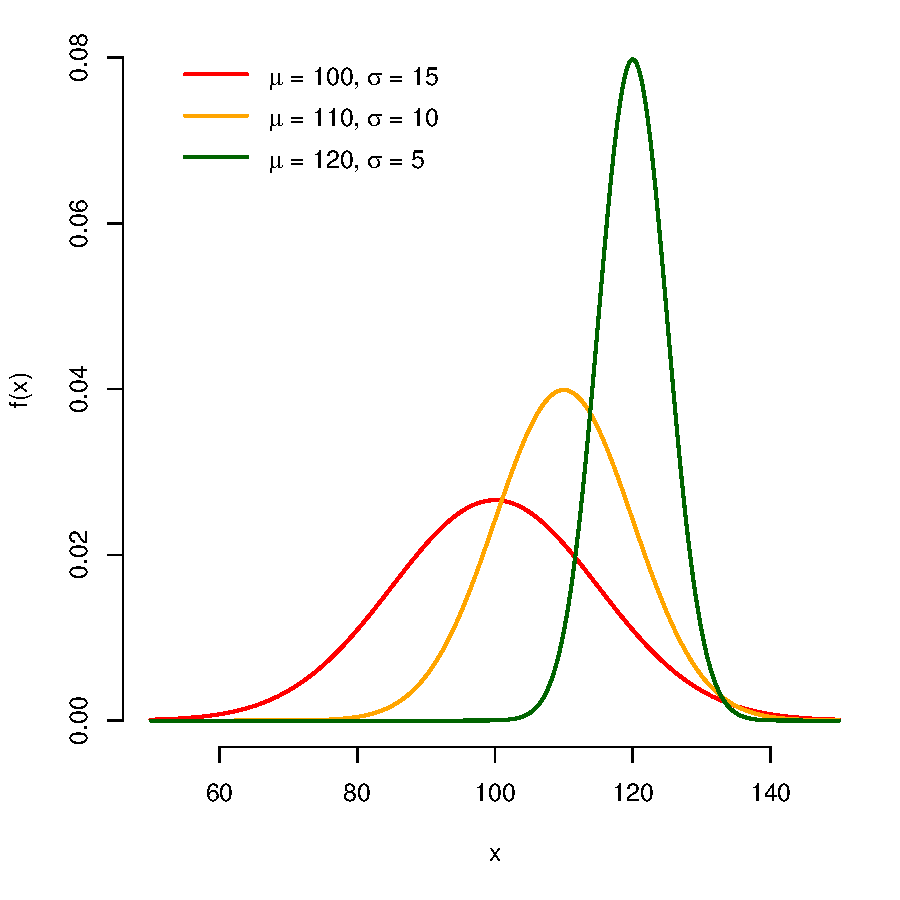
\includegraphics[width=.6\linewidth]{img/ukazka-obr02.pdf}
\caption{A figure with a plot, not entirely related to anything. If you copy the figures from anywhere, always refer to the original author, ideally by citation (if possible). In particular, this picture --- and many others, also a lot of surrounding code --- was taken from the example bachelor thesis of MFF, originally created by Martin Mareš and others.}
\label{fig:g}
\end{figure}

\begin{figure}
\centering
\tikzstyle{box}=[rectangle,draw,rounded corners=0.5ex,fill=green!10]
\begin{tikzpicture}[thick,font=\sf\scriptsize]
\node[box,rotate=45] (a) {A test.};
\node[] (b) at (4,0) {Node with no border!};
\node[circle,draw,dashed,fill=yellow!20, text width=6em, align=center] (c) at (0,4) {Ugly yellow node.\\Is this the Sun?};
\node[box, right=1cm of c] (d) {Math: $X=\sqrt{\frac{y}{z}}$};
\draw[->](a) to (b);
\draw[->](a) to[bend left=30] node[midway,sloped,anchor=north] {flow flows} (c);
\draw[->>>,dotted](b) to[bend right=30] (d);
\draw[ultra thick](c) to (d);

\end{tikzpicture}
\caption{An example diagram typeset with TikZ.}
\end{figure}

\begin{algorithm}
\begin{algorithmic}
\Function{ExecuteWithHighProbability}{$A$}
	\State $r \gets$ a random number between $0$ and $1$
	\State $\varepsilon \gets 0.0000000000000000000000000000000000000042$
	\If{$r\geq\varepsilon$}
		\State execute $A$ \Comment{We discard the return value}
	\Else
		\State print: \texttt{Not today, sorry.}
	\EndIf
\EndFunction
\end{algorithmic}
\caption{Algorithm that executes an action with high probability. Do not care about formal semantics in the pseudocode --- semicolons, types, correct function call parameters and similar nonsense from `realistic' languages can be safely omitted. Instead make sure that the intuition behind (and perhaps some hints about its correctness or various corner cases) can be seen as easily as possible.}
\label{alg:w}
\end{algorithm}

\section{Extra typesetting hints}

Do not overuse text formatting for highlighting various important parts of your sentences. If an idea cannot be communicated without formatting, the sentence probably needs rewriting anyway. Imagine the thesis being read aloud as a podcast --- the storytellers are generally unable to speak in boldface font.

Most importantly, do \underline{not} overuse bold text, which is designed to literally \textbf{shine from the page} to be the first thing that catches the eye of the reader. More precisely, use bold text only for `navigation' elements that need to be seen and located first, such as headings, list item leads, and figure numbers.

Use underline only in dire necessity, such as in the previous paragraph where it was inevitable to ensure that the reader remembers to never typeset boldface text manually again.

Use \emph{emphasis} to highlight the first occurrences of important terms that the reader should notice. The feeling the emphasis produces is, roughly, ``Oh my --- what a nicely slanted word! Surely I expect it be important for the rest of the thesis!''

Finally, never draw a vertical line, not even in a table or around figures, ever. Vertical lines outside of the figures are ugly.
